% $Header: /home/vedranm/bitbucket/beamer/solutions/generic-talks/generic-ornate-15min-45min.de.tex,v 90e850259b8b 2007/01/28 20:48:30 tantau $

\documentclass{beamer}

% Diese Datei enth�lt eine L�sungsvorlage f�r:


% - Vortr�ge �ber ein beliebiges Thema.
% - Vortragsl�nge zwischen 15 und 45 Minuten. 
% - Aussehen des Vortrags ist verschn�rkelt/dekorativ.



% Copyright 2004 by Till Tantau .
%
% In principle, this file can be redistributed and/or modified under
% the terms of the GNU Public License, version 2.
%
% However, this file is supposed to be a template to be modified
% for your own needs. For this reason, if you use this file as a
% template and not specifically distribute it as part of a another
% package/program, I grant the extra permission to freely copy and
% modify this file as you see fit and even to delete this copyright
% notice. 



\mode<presentation>
{
  \usetheme{Frankfurt}
  \setbeamertemplate{footline}[page number]
%   \usetheme{Rochester}
  % oder ...
  %\usecolortheme{crane}
  
  \setbeamercovered{transparent}
  % oder auch nicht
}
\setbeamercolor{alerted text}{fg=green!40!black}

\usepackage[german]{babel}
% oder was auch immer

\usepackage[latin1]{inputenc}
% oder was auch immer
\usepackage{amsmath}
\usepackage{times}
\usepackage[T1]{fontenc}
% Oder was auch immer. Zu beachten ist, das Font und Encoding passen
% m�ssen. Falls T1 nicht funktioniert, kann man versuchen, die Zeile
% mit fontenc zu l�schen.
\usepackage{booktabs}
\usepackage{multirow}
\newcommand{\T}{\ensuremath{^\mathsf{T}}}

\title % (optional, nur bei langen Titeln n�tig)
{Ultrakurze Laserpulse:}

\subtitle
{wie sie helfen die Geheimnisse heterogener Katalyse zu entschl�sseln} % (optional)

\author[] % (optional, nur bei vielen Autoren)
{Robert Scholz}
% - Der \inst{?} Befehl sollte nur verwendet werden, wenn die Autoren
%   unterschiedlichen Instituten angeh�ren.

\institute % (optional, aber oft n�tig)
{AG Saalfrank \\ Institut f�r Chemie \\ Universit�t Potsdam}

%   \inst{1}%
%   Institut f�r Informatik\\
%   Universit�t Hier
%   \and
%   \inst{2}%
%   Institut f�r theoretische Philosophie\\
%   Universit�t Dort}
% - Der \inst{?} Befehl sollte nur verwendet werden, wenn die Autoren
%   unterschiedlichen Instituten angeh�ren.
% - Keep it simple, niemand interessiert sich f�r die genau Adresse.

\date[] % (optional)
{19. April 2017}


%\subject{Informatik}
% Dies wird lediglich in den PDF Informationskatalog einf�gt. Kann gut
% weggelassen werden.


% Falls eine Logodatei namens "university-logo-filename.xxx" vorhanden
% ist, wobei xxx ein von latex bzw. pdflatex lesbares Graphikformat
% ist, so kann man wie folgt ein Logo einf�gen:





% Folgendes sollte gel�scht werden, wenn man nicht am Anfang jedes
% Unterabschnitts die Gliederung nochmal sehen m�chte.
% \AtBeginSubsection[]
% {
%   \begin{frame}[plain]{Outline}
%     \tableofcontents[currentsection,currentsubsection]
%   \end{frame}
% }


% Falls Aufz�hlungen immer schrittweise gezeigt werden sollen, kann
% folgendes Kommando benutzt werden:

%\beamerdefaultoverlayspecification{<+->}



\begin{document}



\begin{frame}[plain]
  \begin{columns}
    \column{1.2\textwidth}
      \titlepage
  \end{columns}



\end{frame}

\section{Einleitung}
  \subsection{Motivation}
\begin{frame}{Motivation: Die Bedeutung heterogener Katalyse}
  \vspace{-0.5 cm}
  \begin{columns}[t]
    \column{0.55\textwidth}
      \begin{block}{Chemische Industrie}
        \begin{itemize}
          \setlength{\itemindent}{-0.5em}
          \item D\"ungemittel
          \begin{itemize}
            \setlength{\itemindent}{-2em}
            \item Haber-Bosch-Verfahren (NH$_3$)
  %           \newline (Ammoniak)
            \item Ostwald-Verfahren (HNO$_3$)
  %           \newline(Salpeters\"aure)
          \end{itemize}
          \item Monomere
          \begin{itemize}
            \setlength{\itemindent}{-2em}
            \item Ethylenoxid, Acryls\"aure, Styrol
          \end{itemize}
        \end{itemize}
      \end{block}
      \vspace{-0.3 cm}
      \begin{figure}
        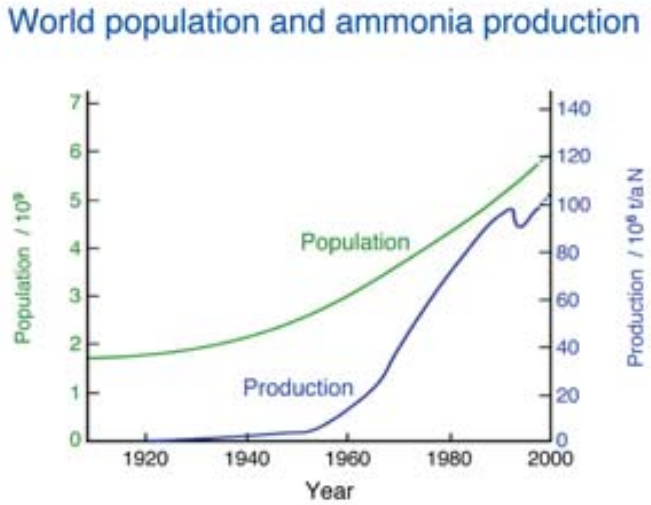
\includegraphics[width = 0.8 \textwidth]{figures/ammonia.png}
      \end{figure}  
      
    \column{0.46\textwidth}  
      \begin{block}{Umwelttechnik}
        \begin{itemize}
          \setlength{\itemindent}{-0.5em}
          \item Luftreinhaltung 
          \begin{itemize}
            \setlength{\itemindent}{-2em}
            \item Abgaskatalysatoren 
            \item Rauchgasentstickung 
          \end{itemize}
          \item Biokraftstoffe
          \begin{itemize}
            \setlength{\itemindent}{-2em}
            \item Fischer-Tropsch-Synthese
          \end{itemize}
        \end{itemize}
      \end{block}

      \vspace{-0.3 cm}
      \begin{columns}[t]
        \column{0.55\textwidth}
          \begin{figure}
            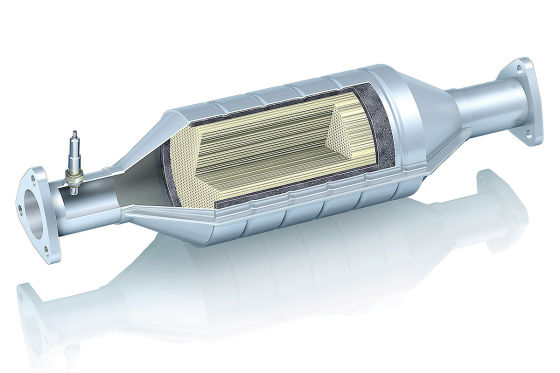
\includegraphics[width = 1.1 \textwidth]{figures/autokat.jpg}
          \end{figure}
        \column{0.5\textwidth}        
          \begin{figure}
            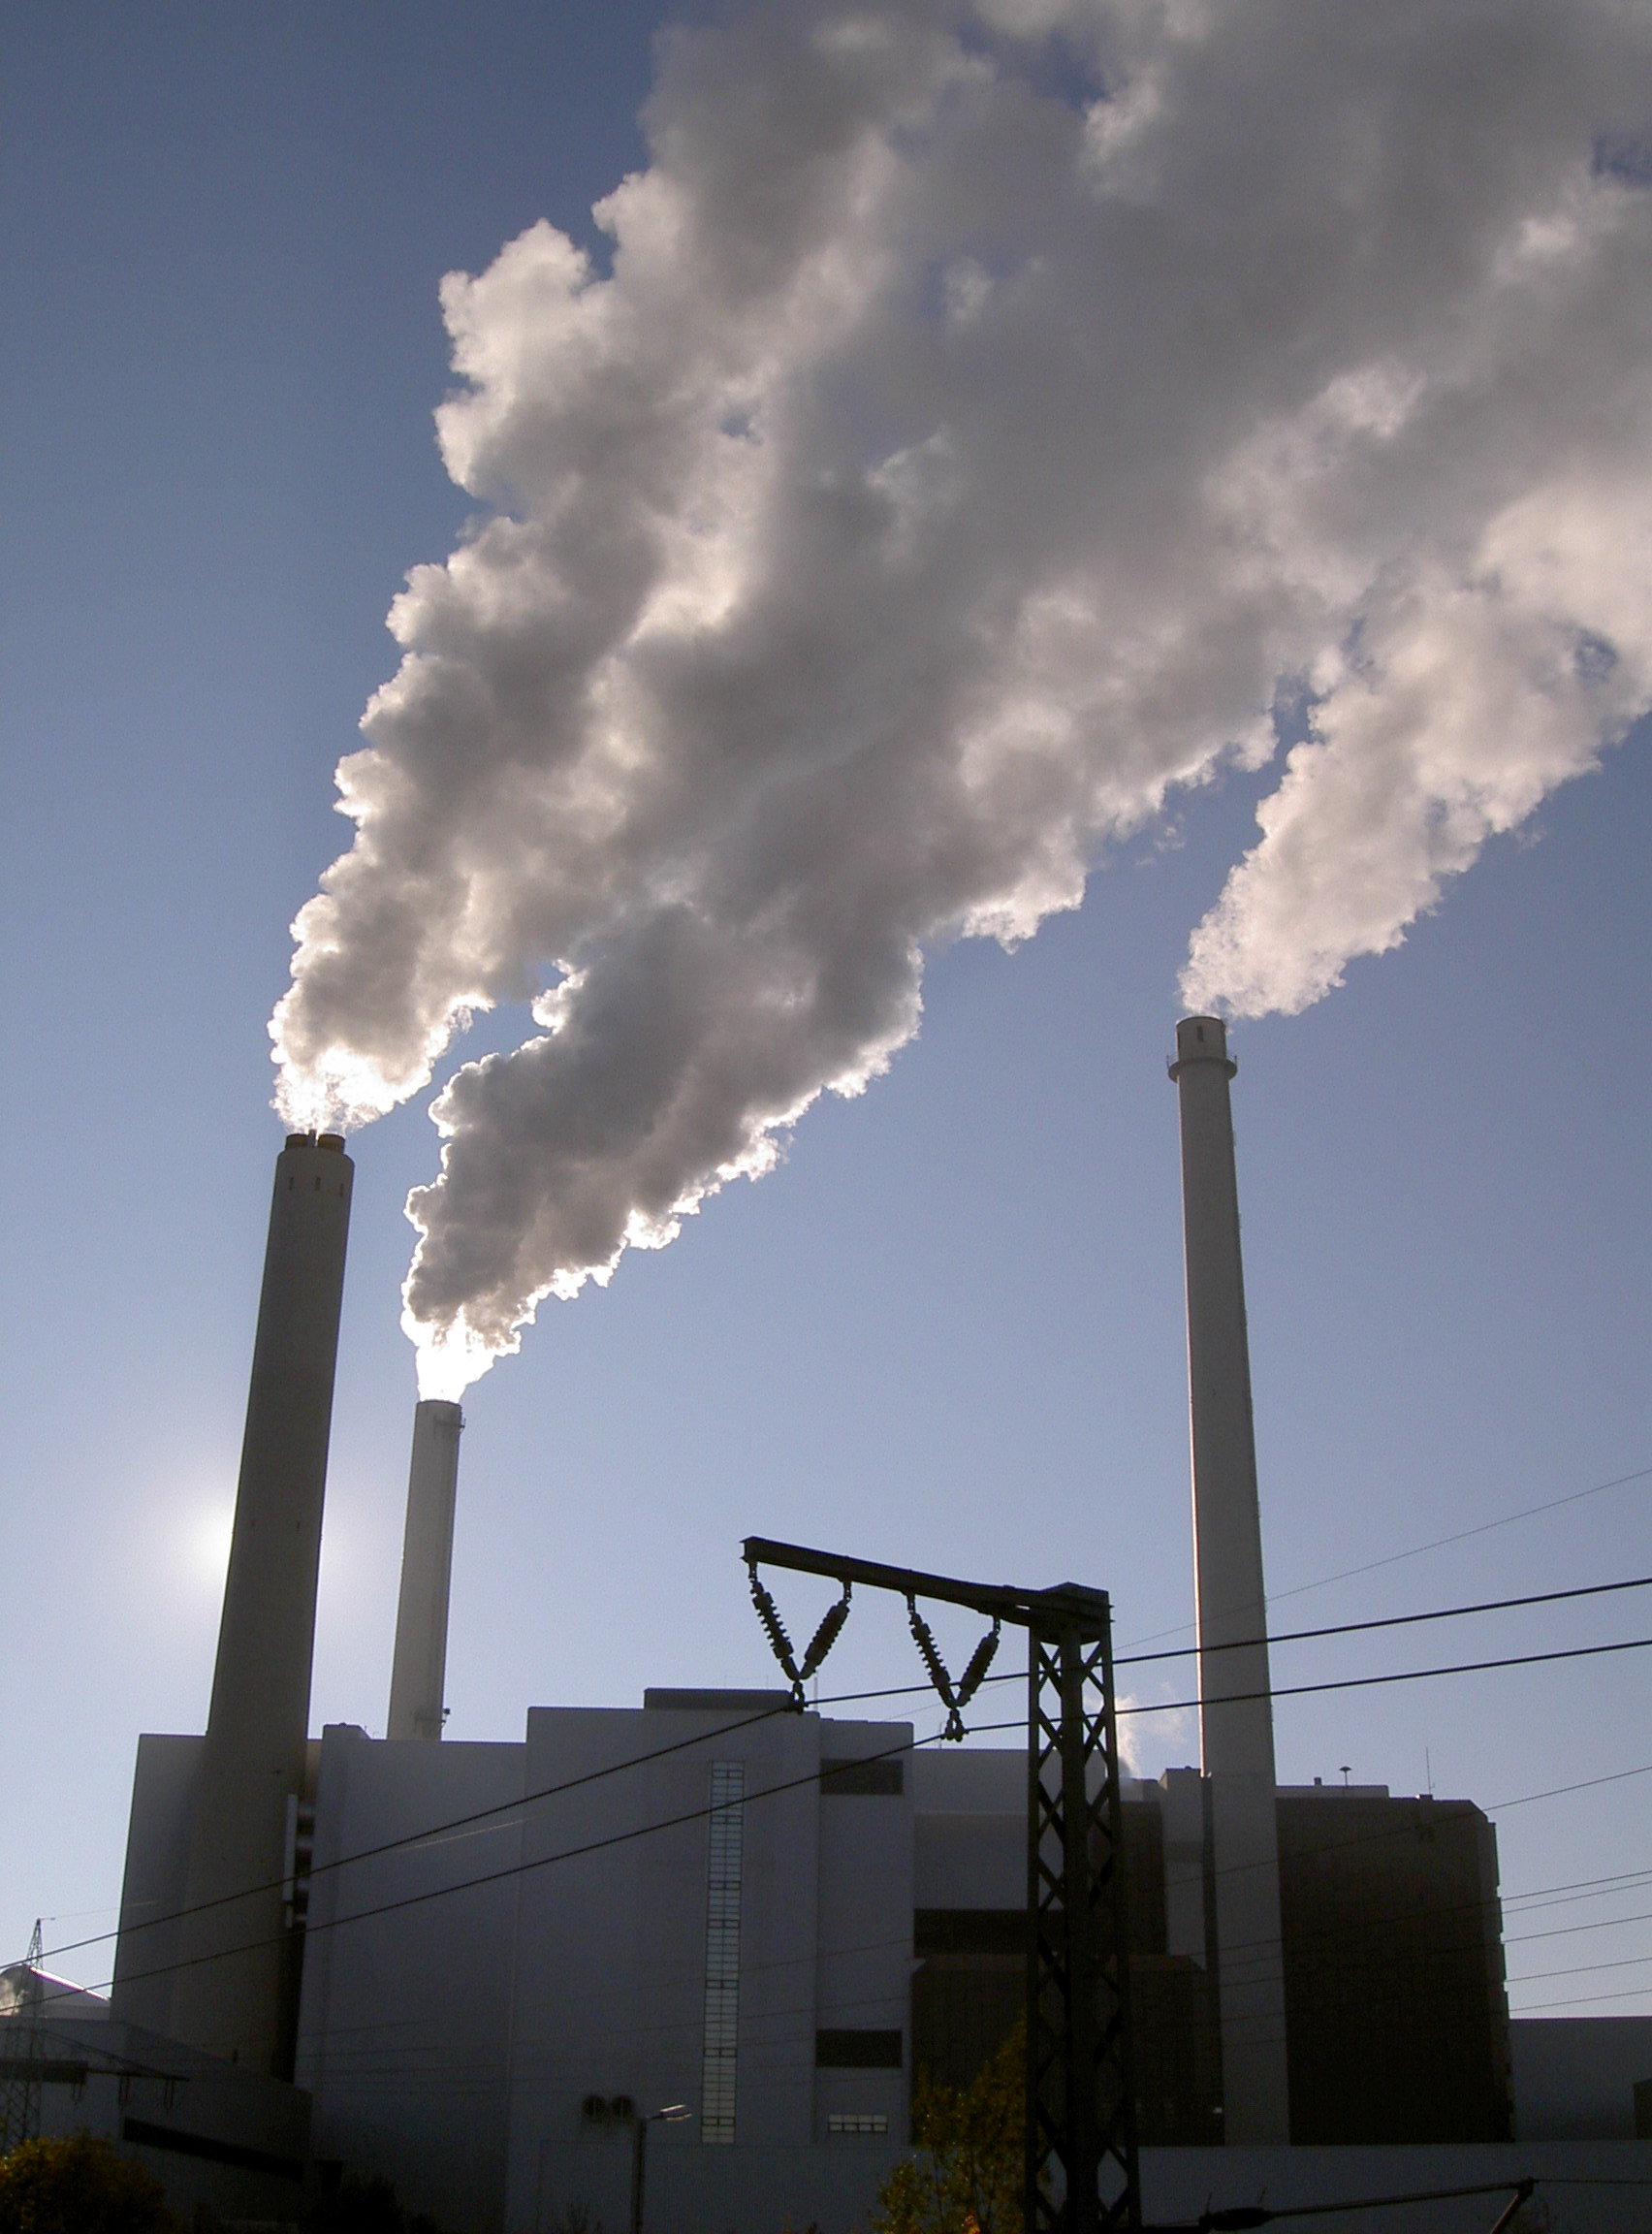
\includegraphics[width = 0.9 \textwidth]{figures/schornsteine.jpg}
          \end{figure}        
      \end{columns}
  \end{columns}
\end{frame}

\begin{frame}{Heterogene Katalyse: Begriffskl\"arung}
  \begin{columns}[t]
    \column{0.5\textwidth}   
      \begin{block}{Katalyse}
        \begin{itemize}
          \item Aktivierungsenergie kleiner \newline $\Rightarrow$ Reaktionen schneller
          \item auch wichtig: Selektivit\"at \newline (z.B. keine Durchoxidation)
        \end{itemize}
      \end{block} 
      
    \column{0.4\textwidth}
      \begin{figure}
        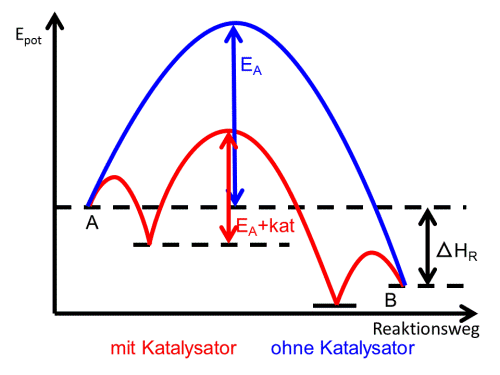
\includegraphics[width=.9\textwidth]{figures/katSchema.png}
      \end{figure}    
  \end{columns}
  
  \begin{block}{Heterogen}
    \begin{itemize}
      \item verschiedene Phasen, meist:
      \begin{itemize}
        \item Katalysator fest
        \item Reaktanden gasf\"ormig / fl\"ussig
      \end{itemize}
    \end{itemize}
  \end{block}
\end{frame}

\begin{frame}{Prinzipieller Mechanismus heterogener Katalyse}
  \begin{columns}
    \column{0.5\textwidth} 
      \begin{block}{z.B. Langmuir-Hinshelwood}
        \begin{enumerate}
             \setlength{\itemindent}{-.5em}
          \item Adsorption Edukte 
          \begin{itemize}
            \setlength{\itemindent}{-2em}
            \item Schw\"achung von Bindungen
            \item ggf. Dissoziation
          \end{itemize}
          \item Oberfl\"achendiffusion
          \item Reaktion 
          \item Desorption Produkt(e)
        \end{enumerate}
      \end{block}
      
    \column{0.5\textwidth} 
%       \vspace{-.1cm}
      \begin{figure}
        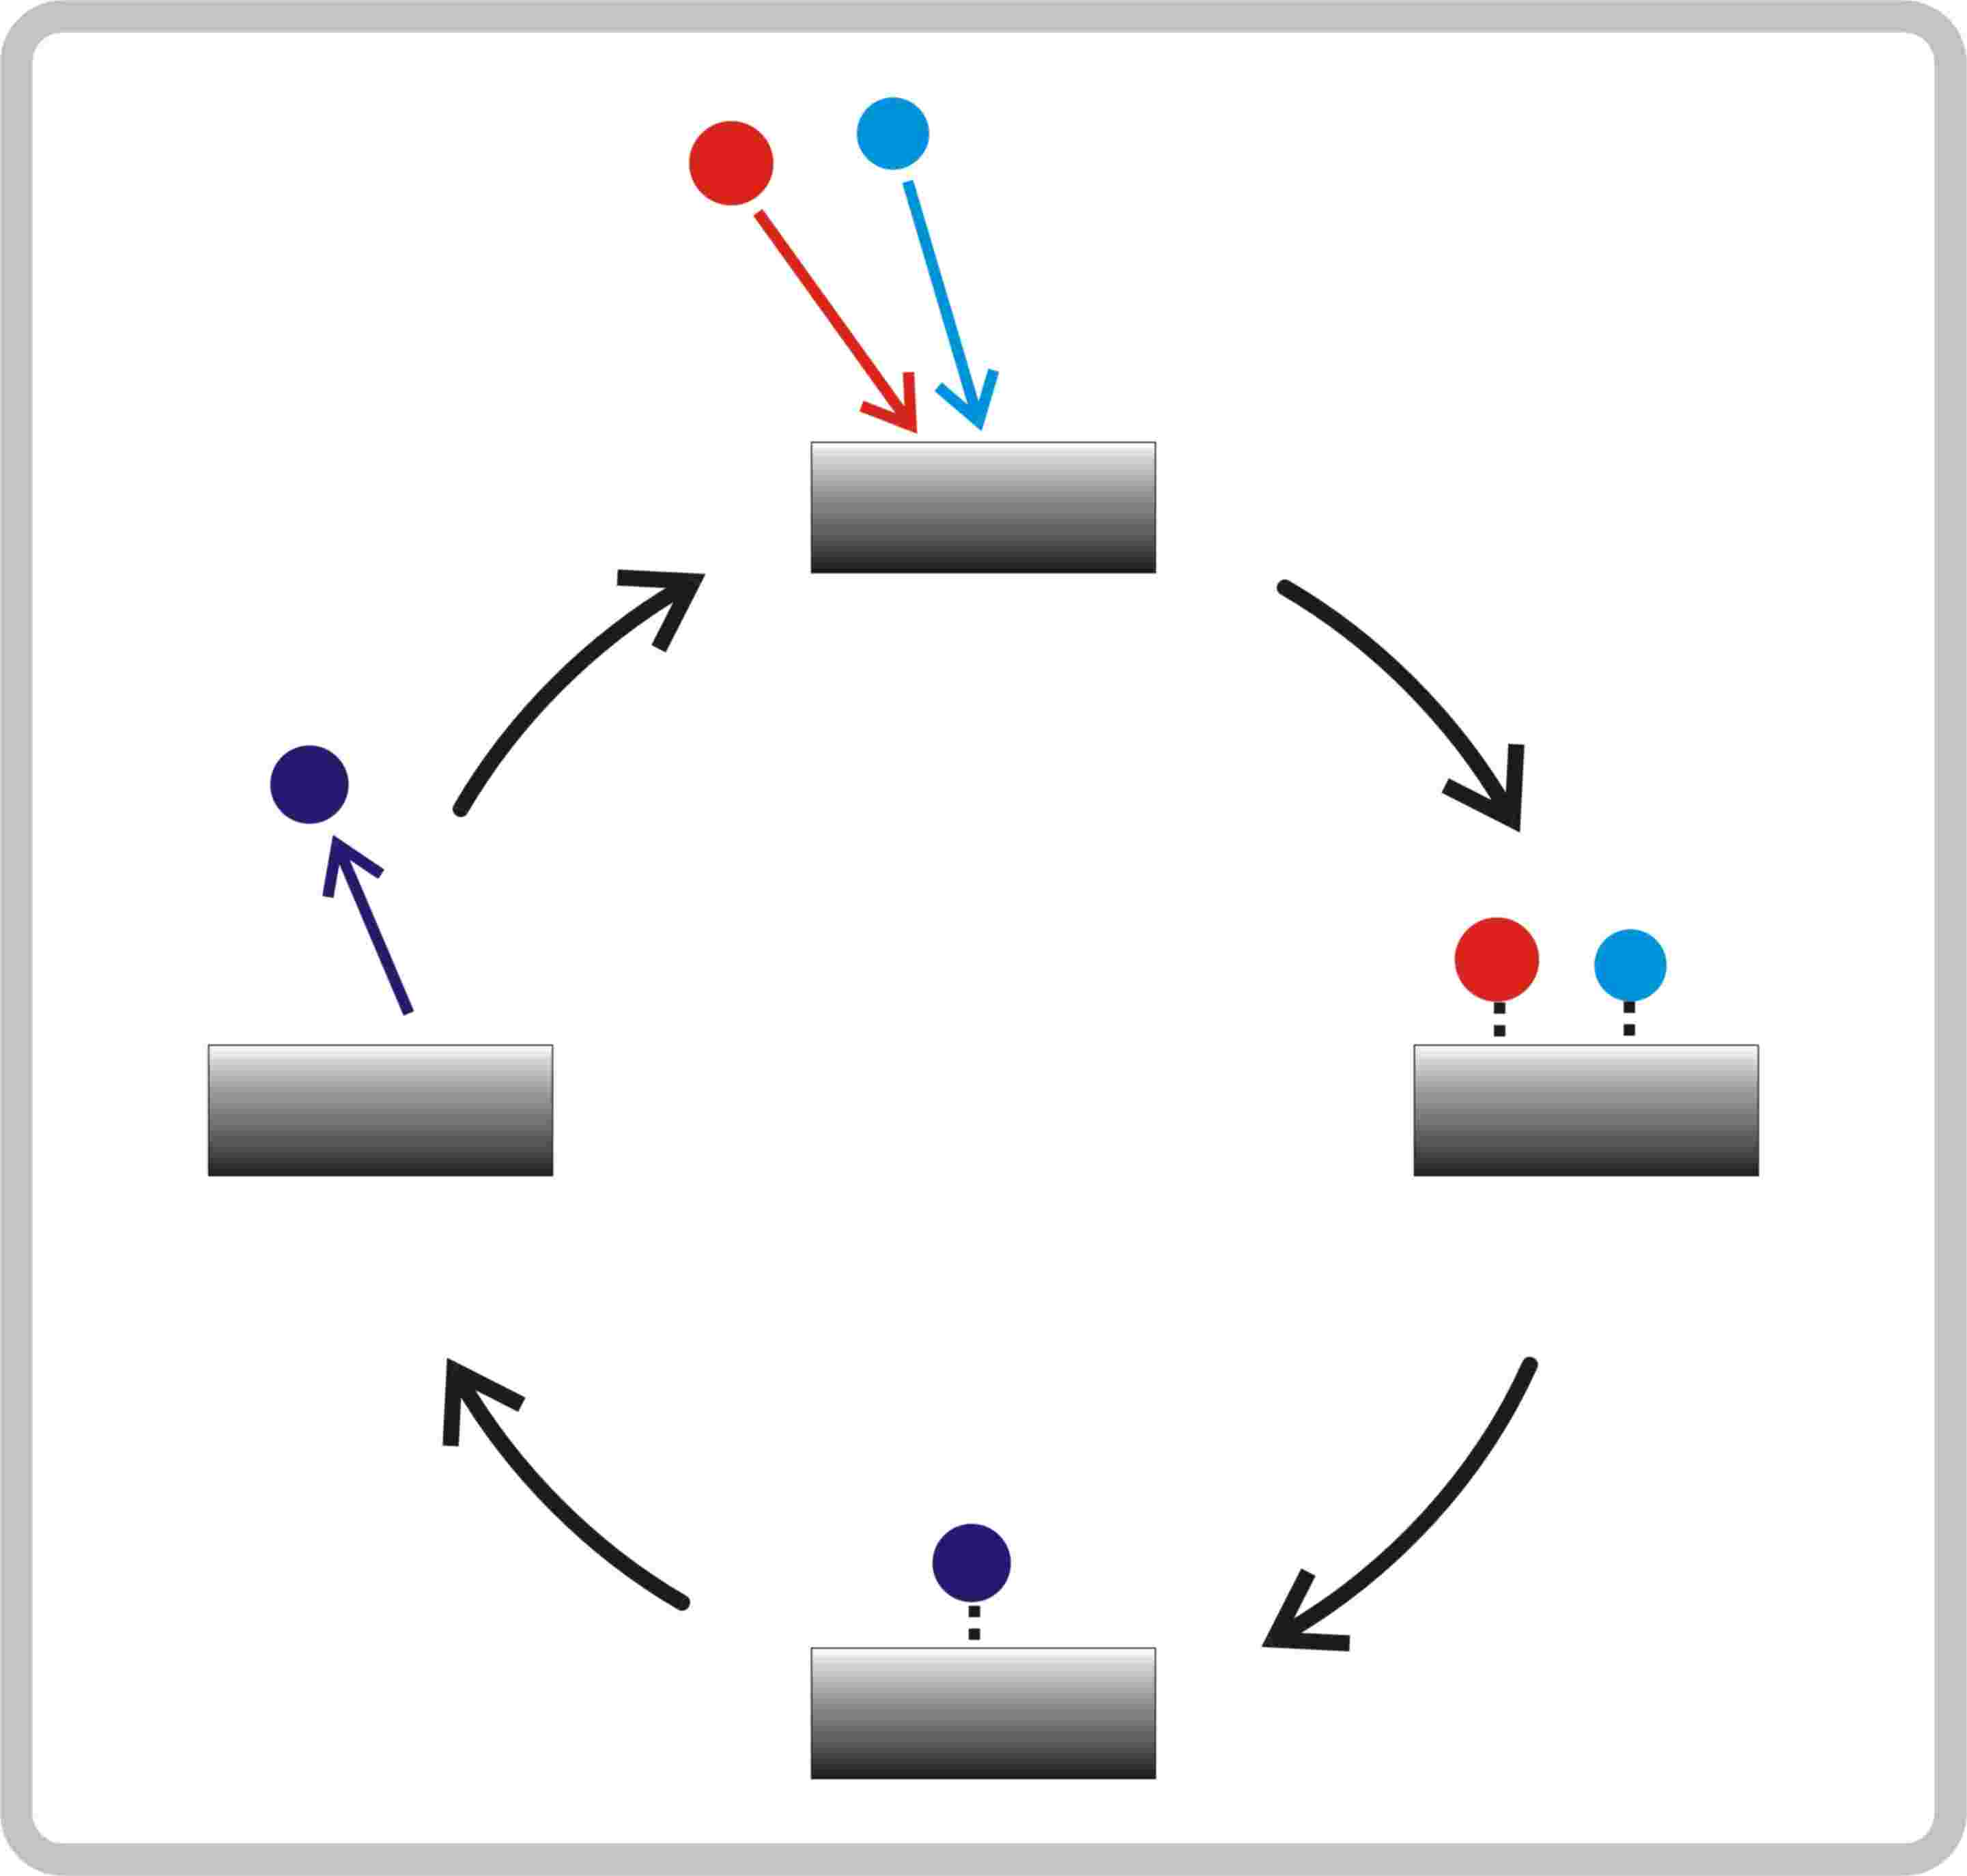
\includegraphics[width = 0.85\textwidth]{figures/langmuir.jpg}
      \end{figure}

  \end{columns}
  \begin{block}{Aber weiterhin viele ungekl\"arte Fragen}
%     \begin{itemize}
      $\Rightarrow$ Grundlagenforschung an Modellsystemen n\"otig
      \begin{itemize}          \setlength{\itemindent}{-.8em}
        \item besonders f\"ur Metall-Adsorbat-Bindung viele Wissensl\"ucken
      \end{itemize}

%     \end{itemize}
  \end{block}

\end{frame}


\section{Theoretische Grundlagen}
\subsection{Theorie}

\begin{frame}{Wie binden Adsorbate an Metalle?}
%   \begin{columns}[t]
    
%   \end{columns}
  \begin{block}{Protonen ``kleben'' an Metalloberfl\"achen}
    \begin{itemize}
      \item Aber, einfaches Sto\ss{}modell: 98$ \%$ Energie erhalten
      \item was fehlt? $\Rightarrow$ Elektronische Reibung!
    \end{itemize}
  \end{block}

  
  \begin{figure}
    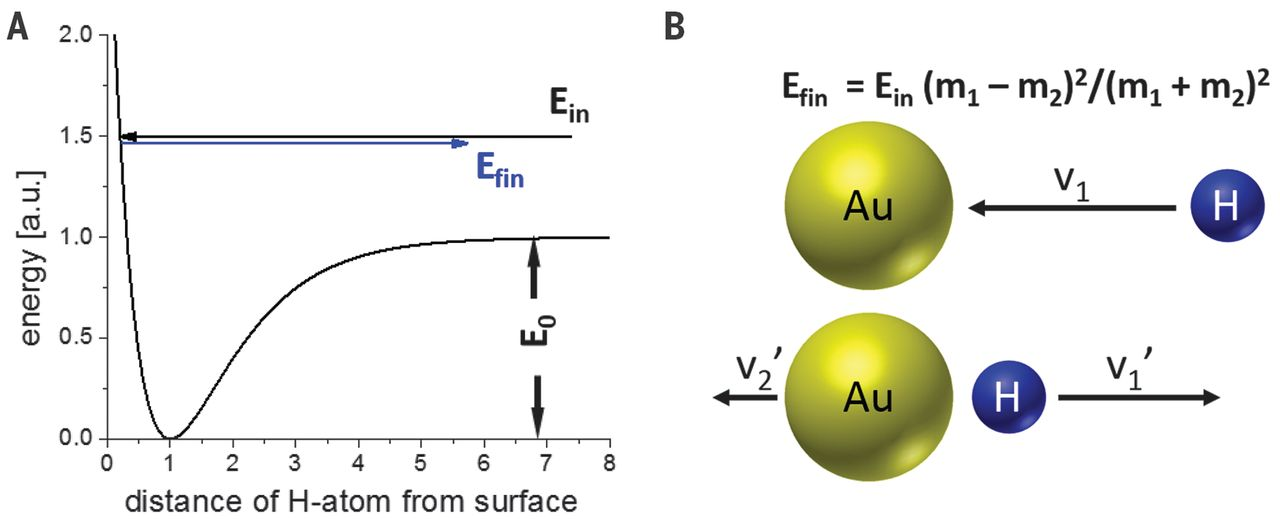
\includegraphics[width = \textwidth]{figures/hgold.jpg}
  \end{figure}

  {\scriptsize \begin{center}
    B\"unermann \textit{et al.}, \textit{Science} 2015 (Prof. Wodtke, G\"ottingen)                                                                 
  \end{center}}
\end{frame}

\begin{frame}{Elektronische Reibung in Metall-Adsorbat-Systemen}
  \begin{block}{Was ist Elektronische Reibung?}
    \begin{itemize}
      \item Wechselwirkung zwischen Adsorbat und Elektronengas 
      \item Ursache: fehlende Bandl\"ucke in Metallen 
      \newline $\Rightarrow$ Anregung von Elektron-Loch-Paaren sehr leicht
    \end{itemize}
  \end{block}
  
  \vspace{-.2cm}
  \begin{columns}[t]
    \column{0.4\textwidth}
      \vspace{-.5cm}
      \begin{figure}
        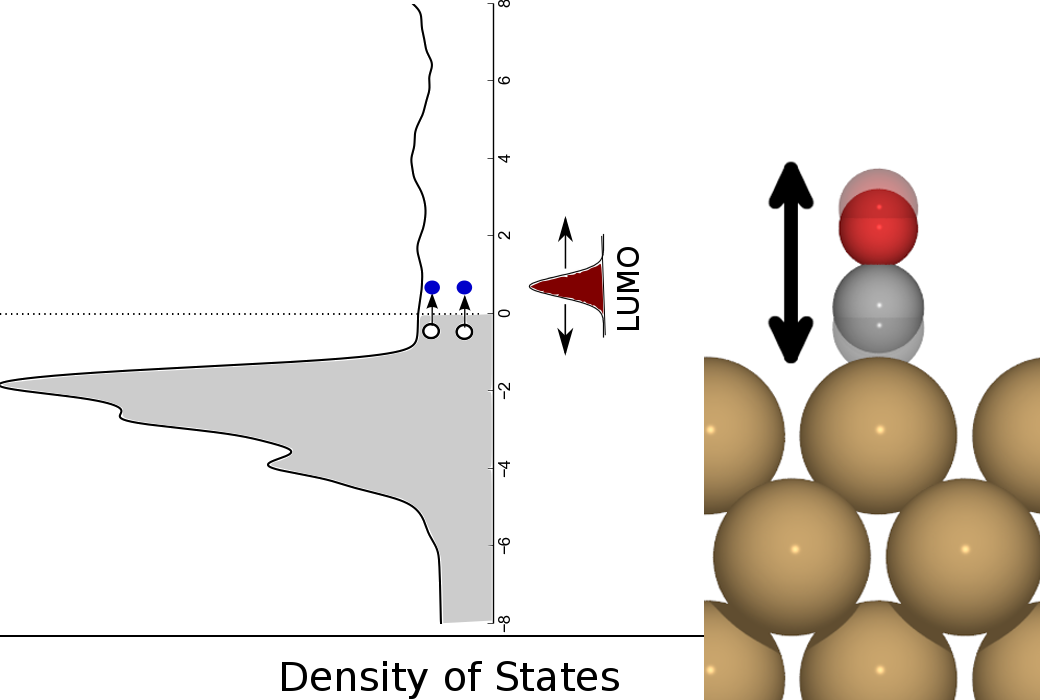
\includegraphics[width = 1.05 \textwidth]{figures/elecFric.png}
      \end{figure}
      {\scriptsize \begin{center}
        Maurer \textit{et al.}, \textit{PRB} 2016 \newline (Prof. Tully, Yale)                                                                 
      \end{center}}
    \column{0.6\textwidth}
      \begin{block}{Was bewirkt elektronische Reibung?}
        \begin{itemize}
          \setlength{\itemindent}{-.5em}
          \item Abremsen von Adsorbaten
          \item starke D\"ampfung von Vibrationen 
          \newline $\Rightarrow$ Lebenszeit $\sim$ ns
          \item umgekehrt, bei hohen Temp.: \newline Fluktuationen $\Rightarrow$ Anregung  
        \end{itemize}
      \end{block}

  \end{columns}

\end{frame}

\begin{frame}{Ultrakurze Laserpulse}
  \begin{columns}[t]
    \column{0.65\textwidth}
      \begin{block}{Einteilung}
        \begin{itemize}
          \item Pikosekundenlaser 
          \begin{itemize}
            \item 1 ps = 10$^{-12}$ s
            \item ab $\approx\,$1 ps Pulsdauer
%             \item lineare Absorption $\propto I$  
          \end{itemize}

          \item Femtosekundenlaser
          \begin{itemize}
            \item 1 fs = 10$^{-15}$ s
            \item typische Pulsdauer: 50 - 200 fs
%             \item nicht-lineare Absorption $\propto I^N$
          \end{itemize}
          \item beide: Spitzenleistung $\gg$ cw-Laser
        \end{itemize}
      \end{block}
      
      \begin{block}{Erforschung elektronischer Reibung}
        \begin{itemize}
          \item Warum reichen ps-Laser nicht?
          \item Was macht fs-Laser besonders?
        \end{itemize}
      \end{block}

    \column{0.3\textwidth}  
    \vspace{.4cm}
    \begin{figure}
      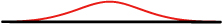
\includegraphics[width = 1. \textwidth]{figures/ps.png}
    \end{figure}
    
    \vspace{-.5cm}
    \begin{figure}
      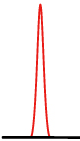
\includegraphics[width = 0.4 \textwidth]{figures/fs.png}
    \end{figure}
    
    \vspace{.2cm}
    \begin{center}
       \Huge\textbf{?}
    \end{center}

  \end{columns}

\end{frame}

\begin{frame}{Wirkung von optischen fs-Lasern auf Metalle}
  \begin{columns}
    \column{0.67\textwidth}
      \begin{block}{Wie wird Energiepuls aufgenommen?}
        \begin{itemize} 
          \setlength{\itemindent}{-.8em}
          \item Nur Elektronen des Metalls absorbieren (Und nur teilweise, Rest: Reflektion)
          \item Elektronen thermalisieren in 10-100 fs
          \newline \hspace*{-.5 cm} $\Rightarrow$ danach Fermi-Dirac-Verteilung f(E)
        \end{itemize}
      \end{block}
      
      \begin{block}{Wie verteilt sich die Energie im Metall?}
        \begin{enumerate}
          \setlength{\itemindent}{-.6em}
          \item Diffusion hei\ss{}er e$^-$ $\Rightarrow$ W\"armetransport
          \item Kopplung zwischen Elektronen und Gitterschwingungen (sog. Phononen)
          \begin{itemize}
            \setlength{\itemindent}{-1.em}
            \item Dauer: ps $\Rightarrow$ \textbf{2 versch. Temperaturen}
            \item anfangs alle Energie in e$^-$-System
            \item da e$^-$ allein geringe W\"armekapazit\"at: \newline
            \hspace*{-1.0 cm} $\Rightarrow$  \textbf{sehr hohe} e$^-$-Temperatur T$_\mathrm{el}> 5000\,$K
          \end{itemize}
        \end{enumerate}
      \end{block}
      
    \column{0.35\textwidth}
      \vspace{-0.7cm}
      \begin{figure}
        \hspace*{.5cm}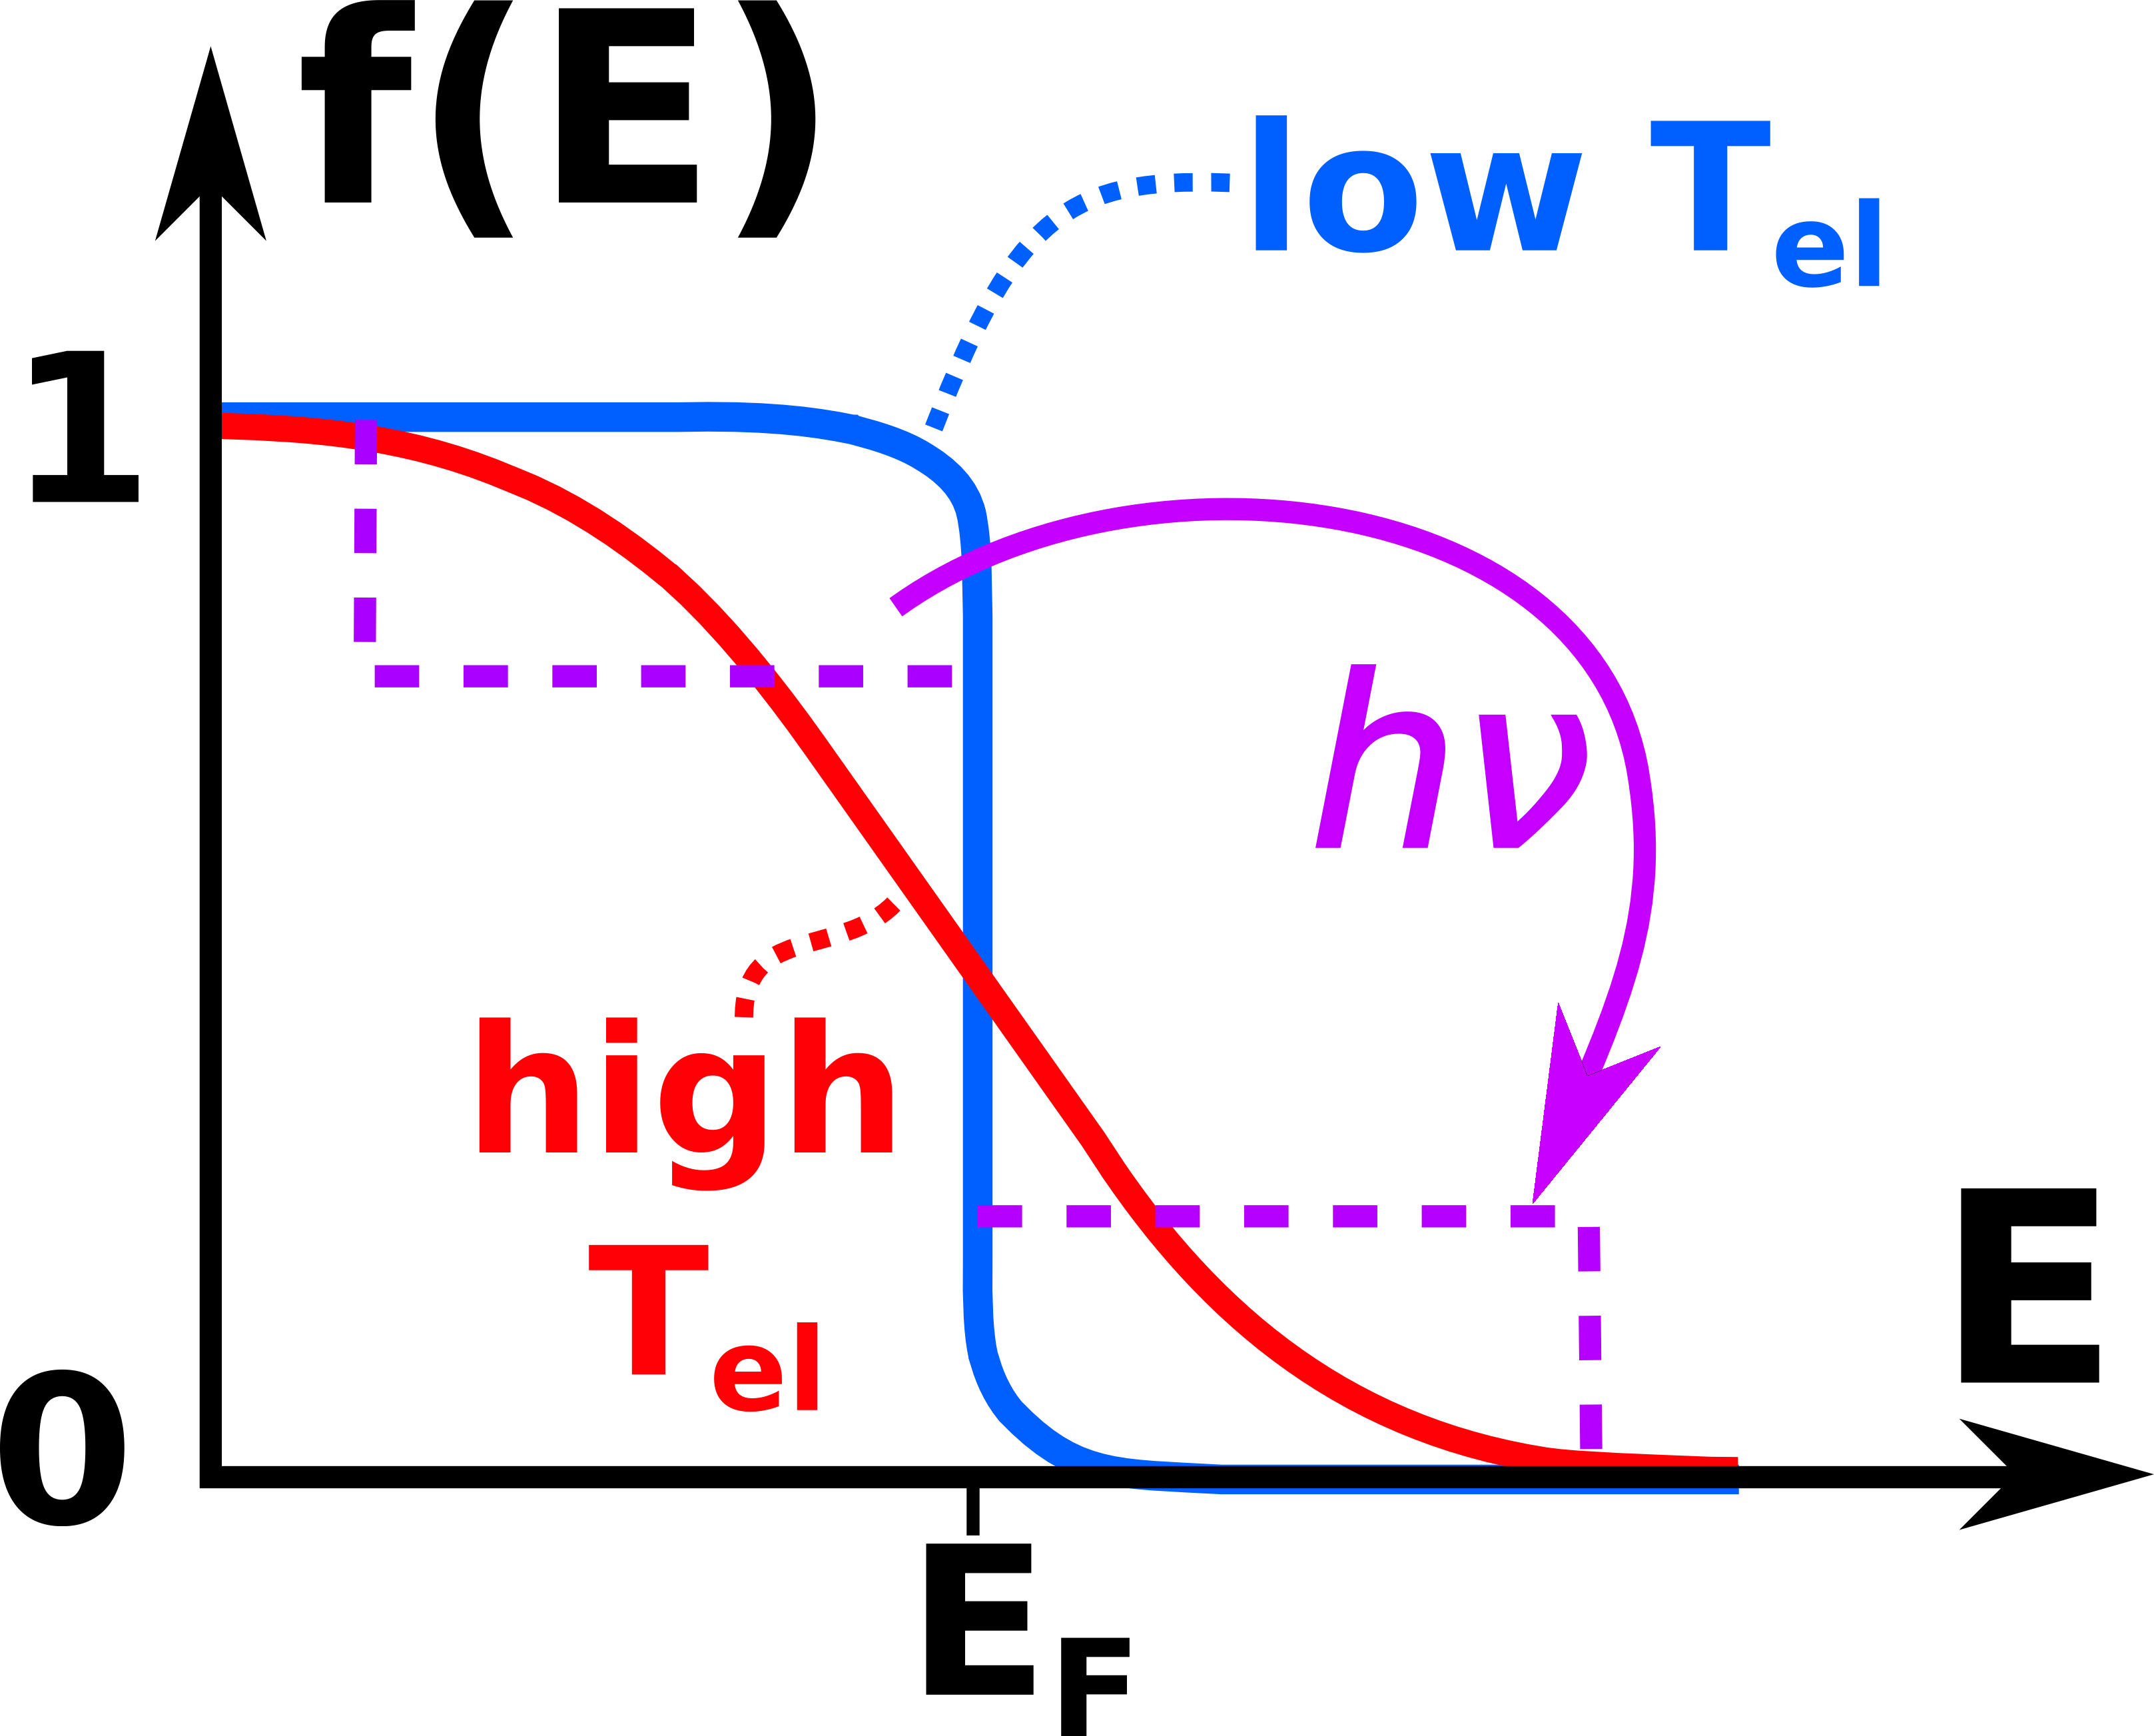
\includegraphics[width = .9\textwidth]{figures/fermi.png}
      \end{figure}

      \vspace{-1.2cm}
      \begin{figure}
        \includegraphics[width = 1.1\textwidth]{figures/TTM_1pulse.eps}
      \end{figure}
      
  \end{columns}


\end{frame}

% \begin{frame}{Zweitemperaturzustand}
%   
% \end{frame}
\begin{frame}{Indirekte Wirkung des fs-Lasers auf Adsorbate}
  \begin{block}{Metall im 2-Temperatur-Zustand wechselwirkt mit Adsorbat}
    \begin{enumerate}
      \item \"uber Elektron-Loch-Paare (e-h-Paare)
        \begin{itemize}
          \item elektronische Reibung (Dissipation)
          \item Anregungen durch hei\ss{}e e-h-Paare (Fluktuation)
          \newline\hspace*{-.5cm} $\Rightarrow$ verursachen Zufallskr\"afte (daher sog. Langevin-Dynamik)
        \end{itemize}
      \item \"uber St\"o\ss{}e mit Phononen 
    \end{enumerate}
  \end{block}
  
  \vspace{-.2cm}
  \begin{figure}
    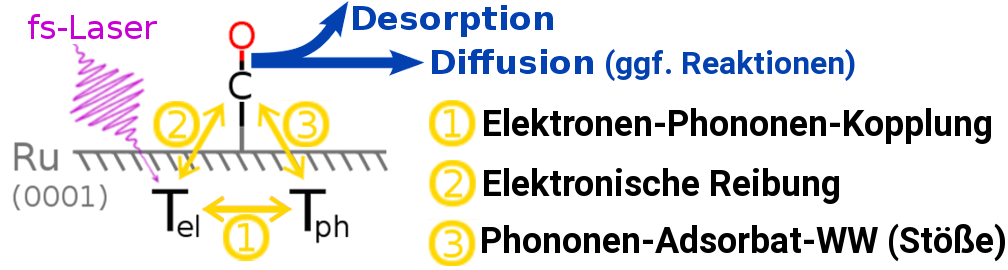
\includegraphics[width = .95\textwidth]{figures/germanSurfScheme.png}
  \end{figure}
  \vspace{-.35cm}
  \begin{block}{Im Folgenden, zwei verschiedene Modelle:}
    ohne (3): \textbf{MDEF}  \hspace{3cm} mit (3): \textbf{MDEF-GLO}
  \end{block}

\end{frame}

\section{Ergebnisse}
\subsection{Ergebnisse}

\begin{frame}{Beispiel CO auf Ru - Diffusion nach Laseranregung}
  \begin{figure}
        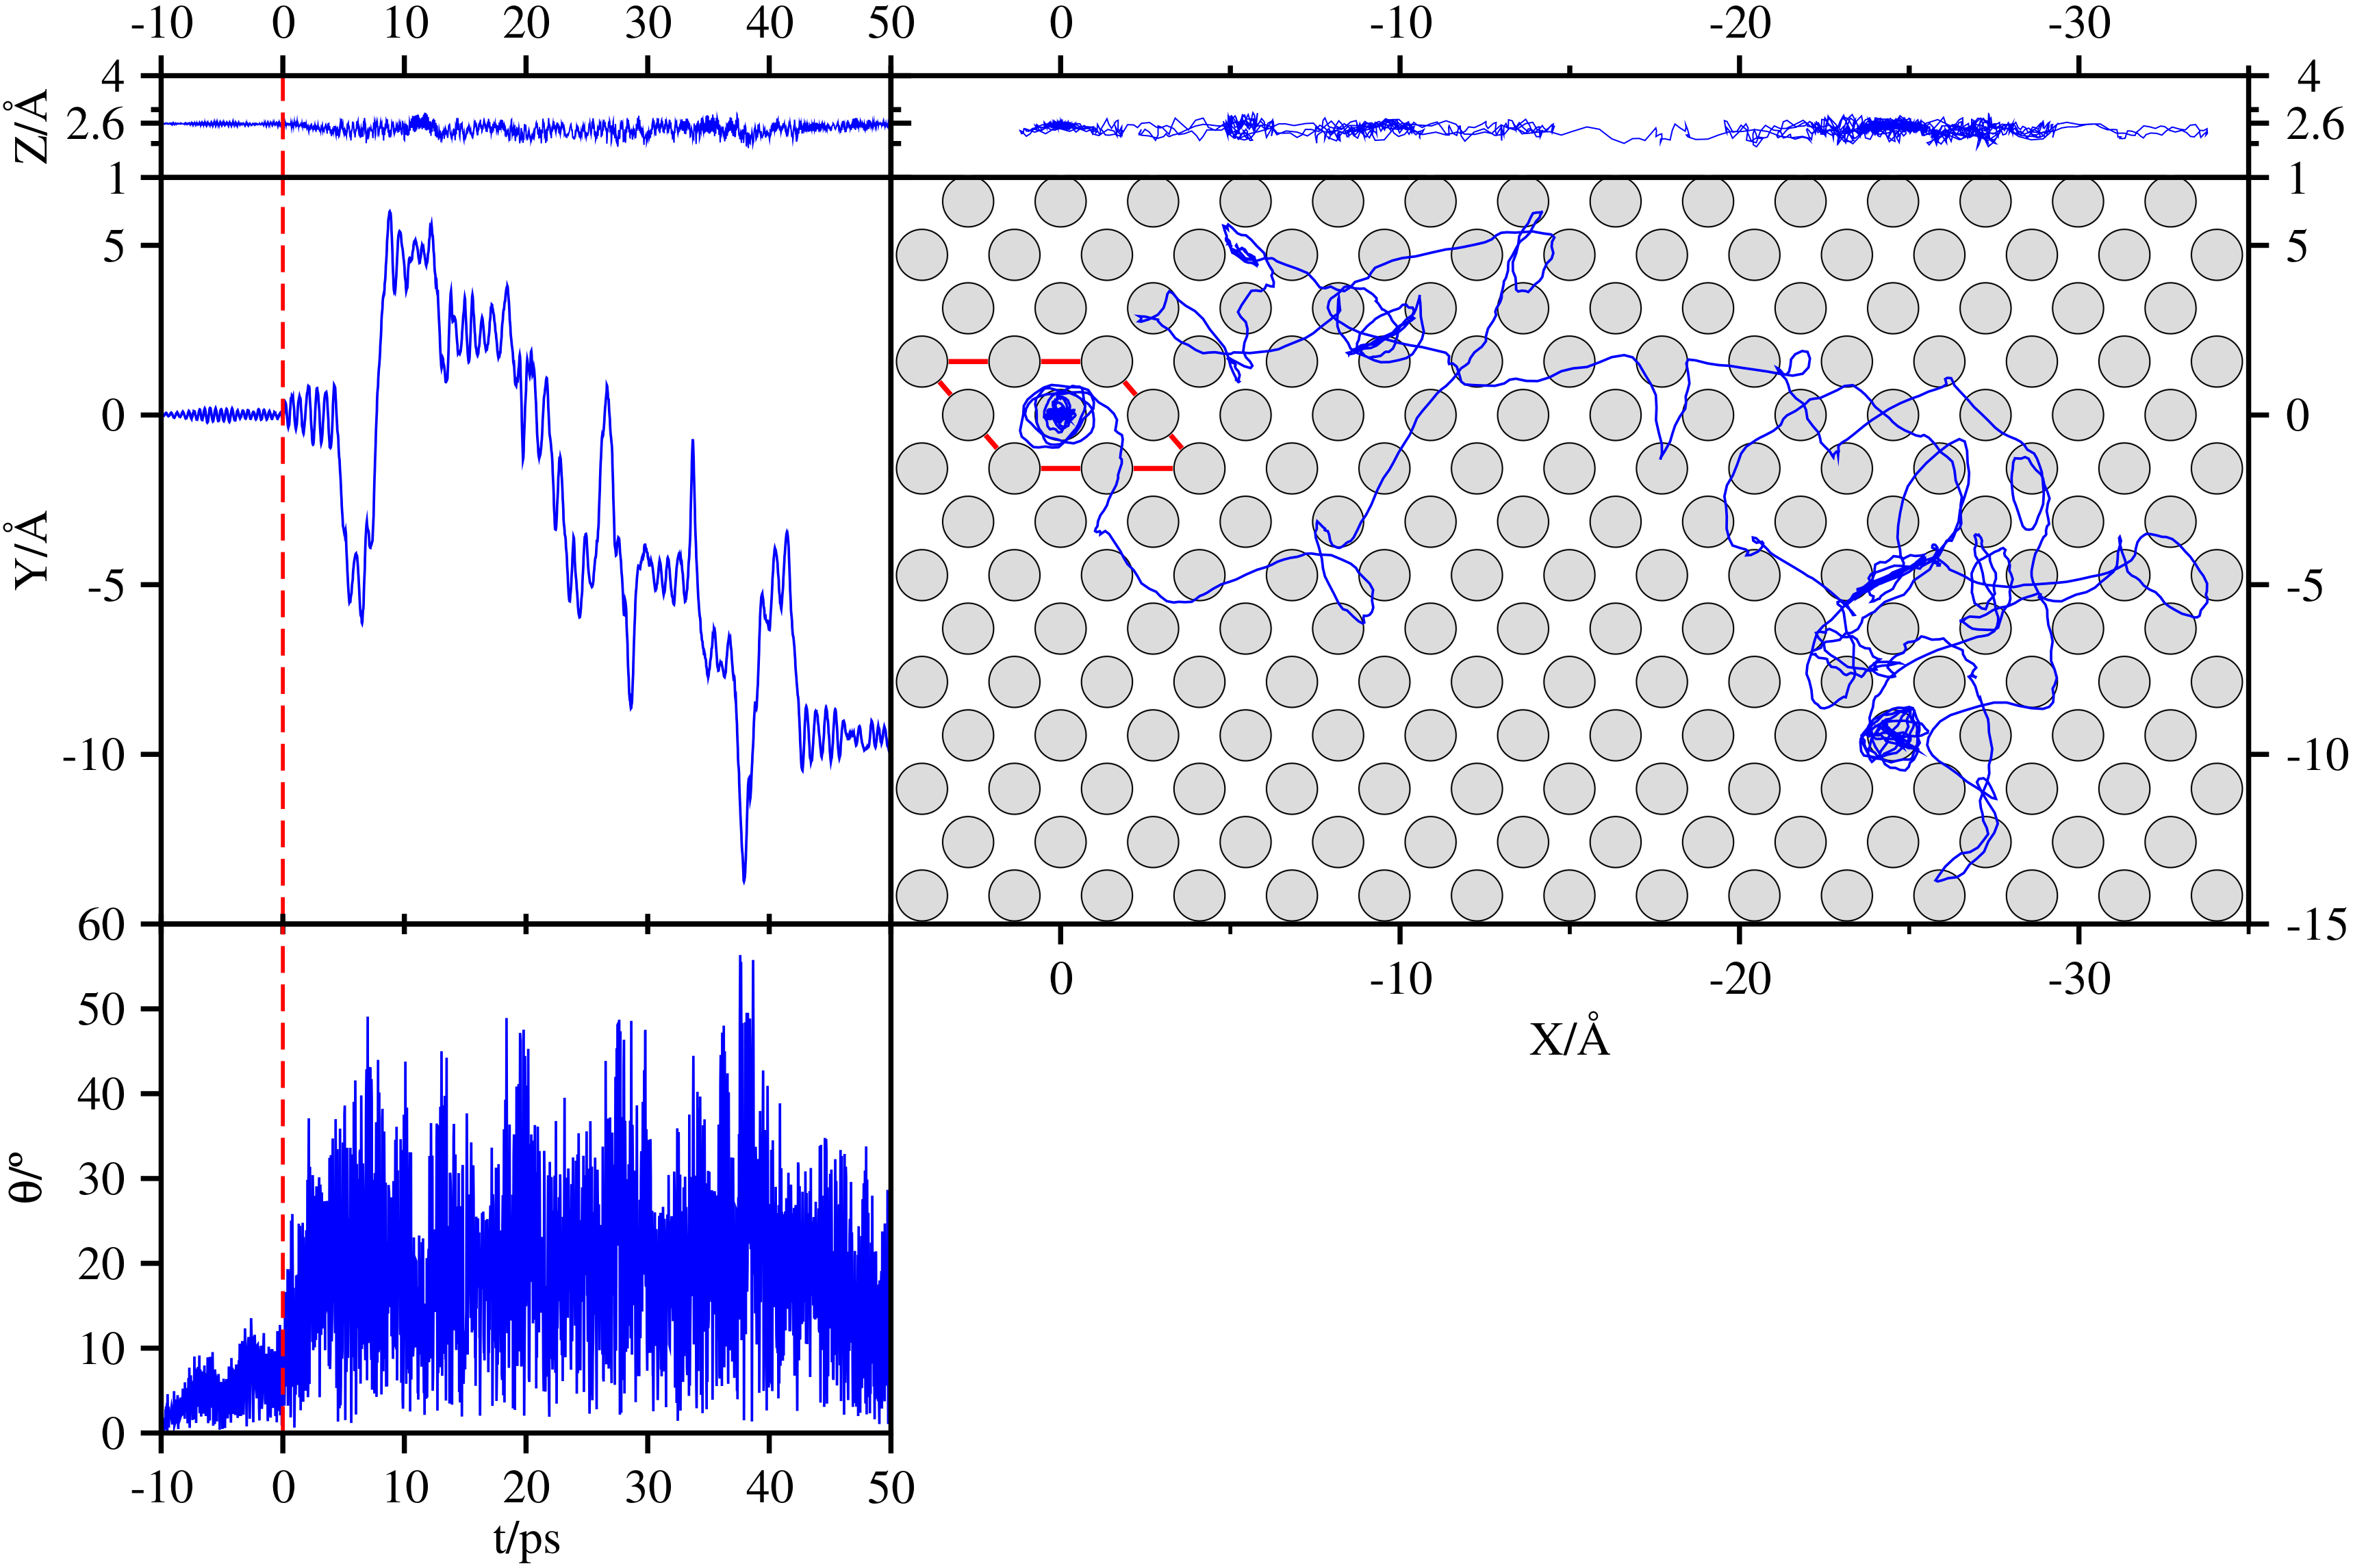
\includegraphics[width=\textwidth]{figures/Traj_XYZTh.png}
  \end{figure}
\end{frame}

\begin{frame}{Beispiel CO auf Ru - Adsorbattemperatur}
  \vspace{-.45cm}
  \begin{columns}[t]
    \column{.65\textwidth}
      \begin{figure}
        \includegraphics[width = 1.\textwidth]{figures/fig_3b.eps}
      \end{figure} 
      \vspace{-.55cm}
      \begin{block}{simulierte Adsorbattemperatur T$_\mathrm{ads}$}
       \begin{itemize}
        \item \"uber je 20000 Trajektorien gemittelt
        \item Vorsicht: keine ``richtige'' Temperatur
        \newline (Verteilung der Energie evtl. anders)
       \end{itemize}
      \end{block}

    \column{.3\textwidth}
      \vspace{-.15cm}
      \begin{figure}
        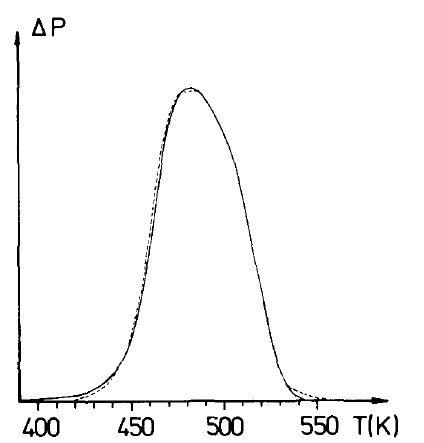
\includegraphics[width = 1.2\textwidth]{figures/TPD.png}
      \end{figure}
      \vspace{-.2cm}
      \begin{block}{TPD-Spektrum}
        \begin{itemize}
         \item Desorption bereits ab 450K erwartet
        \end{itemize}
      \end{block}

  \end{columns}
\end{frame}

\begin{frame}{Beispiel CO auf Ru - Lasergetriebene Desorption}
  \begin{columns}
    \column{0.5\textwidth}
      \begin{block}{Desorption vs. Laserfluenz (doppelt logarithmisch)}
        \begin{itemize}
          \setlength{\itemindent}{-1.em}
          \item folgt grob Potenzgesetz
                $P_\mathrm{des} = A\cdot F^n$
          \item MDEF-GLO: Werte zu hoch, daf\"ur aber fast korrektes $n$
          \item MDEF: $n$ stark abweichend \newline \hspace*{-.8cm} $\Rightarrow$ \"ubersch\"atzt Nicht-Linearit\"at
        \end{itemize}
      \end{block}
    \column{0.55\textwidth}  
      \begin{figure}
        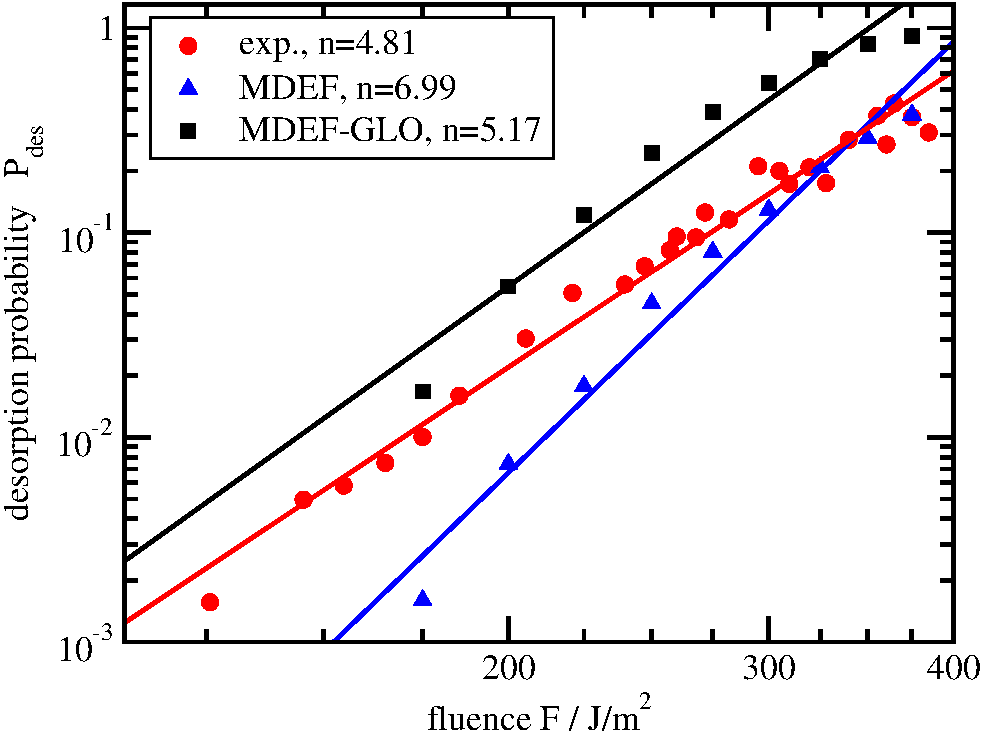
\includegraphics[width=1\textwidth]{figures/Pdes_vs_Fluence.pdf}
      \end{figure}      
  \end{columns}
\end{frame}

\begin{frame}{Beispiel CO auf Ru - ``dynamischer Fallen-Effekt''}
  
%     \begin{figure}
      \hspace*{-.6cm}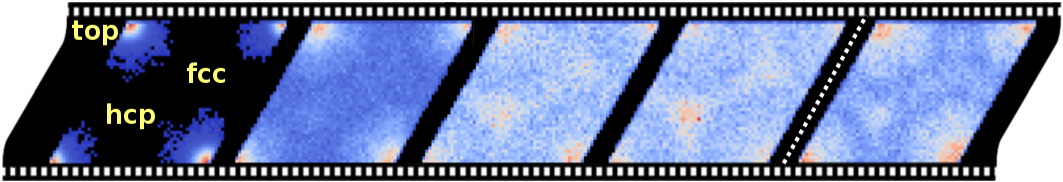
\includegraphics[width=1.1\textwidth]{figures/movie.png}
%     \end{figure}
% \vspace*{-.5cm}
      \begin{columns}[t]
  \column{.6\textwidth}
  \begin{block}{\"Uberraschende Muster in XY-Ebene}
    \begin{itemize}
      \item vor Laser: alle Molek\"ule auf \textbf{top} 
      \item nach 5 ps: \textbf{hcp}-Stelle bevorzugt  
%       \item[$\Rightarrow$] 
      \newline obwohl lokales Maximum!
      \newline $\Rightarrow$ ``dynamical trapping'' 
      \item 30 ps: wieder abgek\"uhlt
      \newline $\Rightarrow$ \textbf{top}-Stelle wieder favorisiert 
    \end{itemize}   
  \end{block}

  \column{.45\textwidth}
    \begin{figure}
      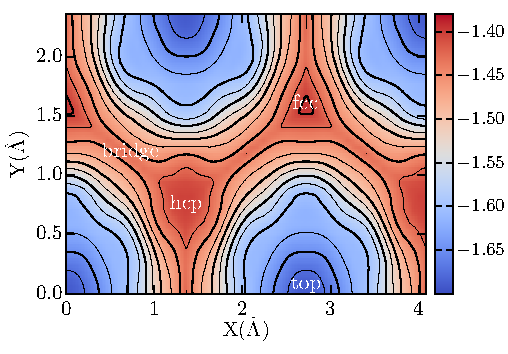
\includegraphics[width=\textwidth]{figures/PES_XYview.pdf}
    \end{figure}
  \end{columns}  
\end{frame}


\section{Zusammenfassung}
  \subsection{Outlook}
\begin{frame}{Zusammenfassung und Ausblick}
  \begin{block}{Zusammenfassung}
    \begin{itemize}
      \item Grundlagenforschung um Katalyse tiefer zu verstehen
      \item Adsorbate auf Metallen unterliegen elektronischer Reibung
      \item fs-Laserpulse regen zun\"achst nur Elektronen an 
      \item hohe Elektronentemperaturen T$_\mathrm{el}$ $\Rightarrow$ Adsorbatdynamik 
    \end{itemize}

  \end{block}
  \begin{block}{Ausblick}
    \begin{itemize}
      \item andere Systeme, z.B. CO/Cu, NO/Au, H$_2$/D$_2$/Ru
      \item Verbesserungen der Methoden, z.B. Reibung, 2T-Modell
      \item komplexeres Modell, z.B. mehrere Adsorbatmolek\"ule 
    \end{itemize}

  \end{block}

\end{frame}  
  
\begin{frame}{Danksagung}
  \begin{columns}[t]
    \column{0.85\textwidth}
      \begin{block}{Vielen Dank... }
        \begin{itemize}
          \item ... f\"ur die wunderbare Betreuung, sowohl fachlich als auch menschlich, an Prof. Peter Saalfrank!
          \item ... f\"ur die tolle Arbeitsatmosph\"are an die gesamte Arbeitsgruppe, insbesondere B\"uro D2.04/05!        
        \end{itemize}
       
      \end{block}
      



    \column{0.2\textwidth}
      \begin{figure}
        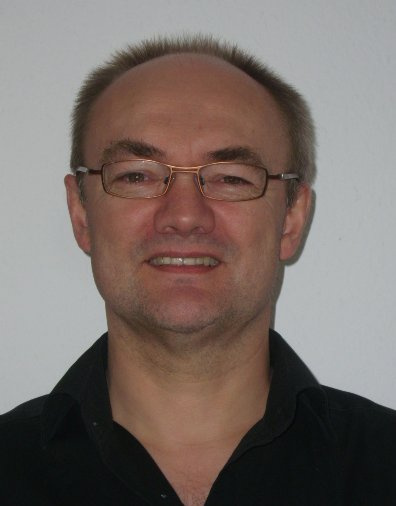
\includegraphics[width = .8 \textwidth]{figures/saalfrank_picture.jpg}
      \end{figure}

  \end{columns}
  
        \begin{block}{}
\Large Und euch vielen Dank f\"ur die Aufmerksamkeit!
      \end{block}

\end{frame}
  
\appendix

\begin{frame}{Further specific motivation for investigating CO/Ru}{F\"uchsel \textit{et al.}, \textit{JChemPhys} 2014} 
  \vspace*{-.4cm}
  \begin{columns}
        \column{.5\textwidth}
          \begin{figure}
                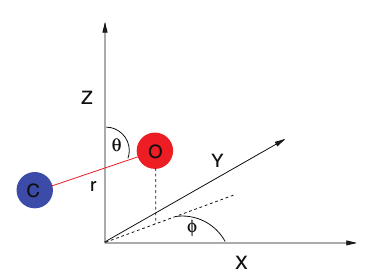
\includegraphics[width=.8\textwidth]{figures/6dimScheme.png}
          \end{figure}
        \column{.5\textwidth}
          \begin{figure}
                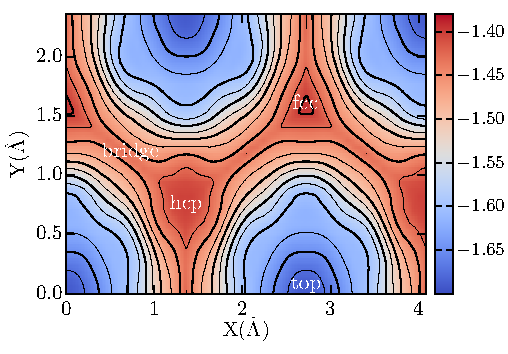
\includegraphics[width=.8\textwidth]{figures/PES_XYview.pdf}
          \end{figure}
        
  \end{columns}
  \begin{block}{Important prior theory work was done at our group \newline{\scriptsize F\"uchsel \textit{et al.}, \textit{JChemPhys} 2014}}
  \begin{itemize} 
    \item Development of a potential energy surface (PES)
          \begin{itemize}
            \item \footnotesize from over 90$\,$000 DFT points!
                \item all 6 dimensions of the adsorbate
    \item very fast because preconstucted\\~
    \item[\LARGE$\Rightarrow$] {\large\textbf{enables large-scale dynamics!}}
          \end{itemize}
  \end{itemize}
  \end{block}
\end{frame}

\begin{frame}{Details of the time-resolved x-ray experiment}{Dell'Angela \textit{et al.}, \textit{Science} 2013 {\scriptsize (experimental part by Nilsson group, SLAC/LCLS, Stanford)}}
  \vspace*{-.7cm}
  \begin{columns}[t]
    \column{0.51\textwidth}
      \begin{block}{What was done?}
        \begin{itemize}
         \item pump: \textit{vis}-fs-laser 
         \item probe: x-ray free $e^{-}$ laser
                  \begin{itemize}\footnotesize
                    \item K-edge of O-atom
                  \end{itemize} 
        \end{itemize}

      \end{block}
%       \begin{block}{How does it work?}
%        
%       \end{block}       
      \begin{block}{What is observed?}
        \begin{itemize}
          \item orbital density of states at O 
          \item energies shift towards gas-phase values of CO
          \item intensities change 
          \begin{itemize}
                \footnotesize
           \item 2$\tilde{\pi}^*$ $\Rightarrow$ increase by $\sim30$\% 
           \item \~{d}$_\pi$ $\,\Rightarrow$ decrease by $\sim30$\%
           \item participator peak appears
          \end{itemize}
          \large \item[\LARGE$\Rightarrow$] physisorbed precursor(?)
        \end{itemize}     
      \end{block}      
    \column{0.50\textwidth}
     \vspace*{-.8cm}
  \begin{figure}
    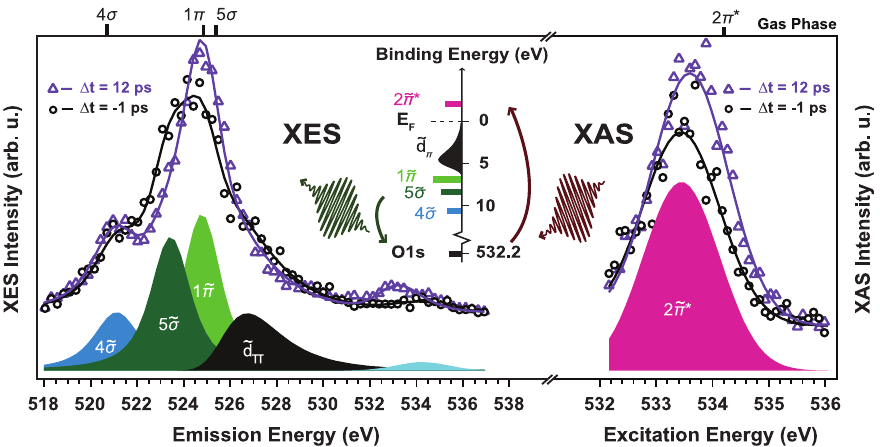
\includegraphics[width=1.1\textwidth]{figures/scienceXray.png}
  \end{figure}
         \vspace*{-.15cm}
%   \begin{figure}
    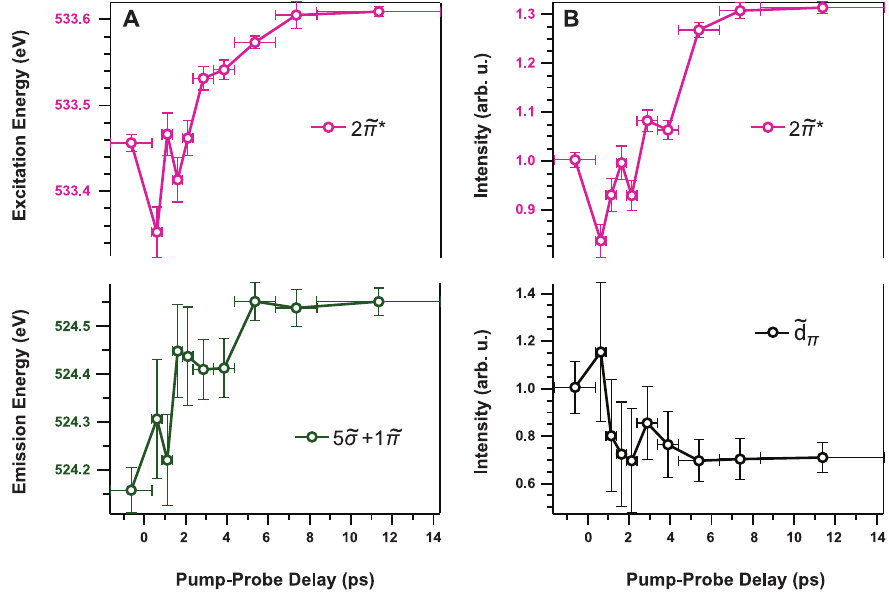
\includegraphics[width=1.1\textwidth]{figures/XrayIntOverTime.png}
%   \end{6figure}
  \end{columns}
\end{frame}

\begin{frame}{More facts about the potential energy surface (PES)}
  \begin{columns}
   \column{0.9\textwidth}
     
  \begin{block}{How was it constructed?}
    \begin{itemize}
      \item GGA-level (RPBE) with VdW-correction (D2)

      \item (2x2) cell with 1 CO $\Rightarrow$ 14 atoms, 0.25 ML coverage
      \begin{itemize}
        \item \footnotesize all 6 dimensions of adsorbate $\Rightarrow$ surface atoms frozen
      \end{itemize} 
      \item interpolation with cubic splines and\newline corrugation reducing procedure (CRP)
      \begin{itemize}
        \item \footnotesize atomic potentials temporarily substracted \newline $\Rightarrow$ smoother intermittent potential, interpolates better
      \end{itemize}
      \item slightly newer PES: C$_{3v}$- instead of C$_{6v}$-symmetry  
      \begin{itemize}
        \item \footnotesize differences between hcp and fcc sites not neglected
      \end{itemize}
     \end{itemize}

  \end{block}
  
   \column{0.15\textwidth}
       \begin{figure}
        \hspace*{-.2cm}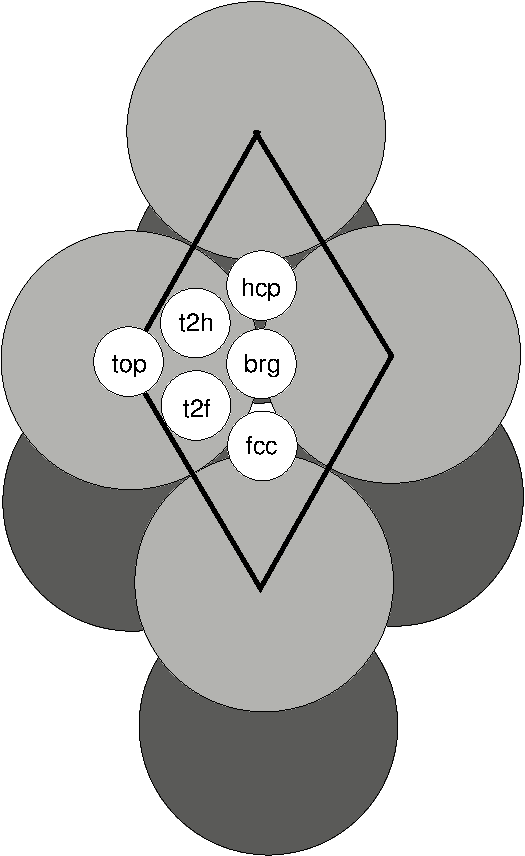
\includegraphics[width=1.3\textwidth]{figures/PES_samplepoints.pdf}
      \end{figure}
      
%       \begin{figure}
%       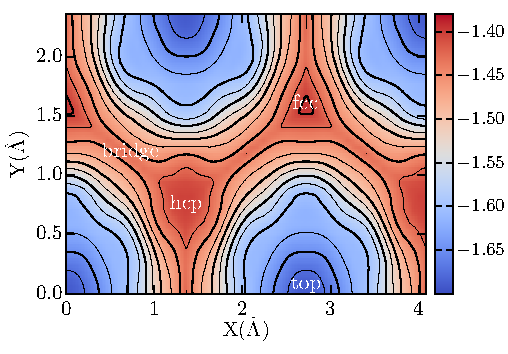
\includegraphics[width=1.2\textwidth]{figures/PES_XYview.pdf}
%       \end{figure}

  \end{columns}
        \begin{figure}
        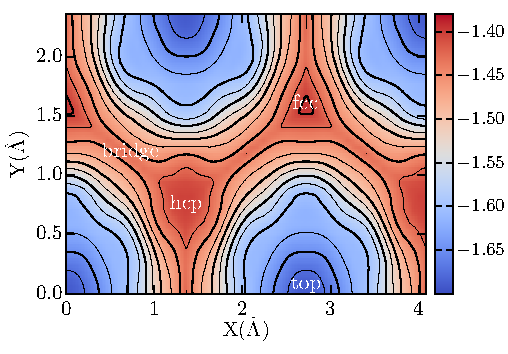
\includegraphics[width=0.33\textwidth]{figures/PES_XYview.pdf}
      \end{figure}
\end{frame}

\begin{frame}{Two-temperature model (TTM)}{Two coupled heat diffusion equations}
  
  \begin{columns}
   \column{0.3\textwidth}
    \begin{figure}
        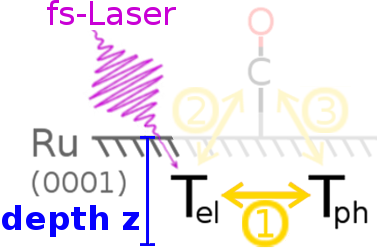
\includegraphics[width=1\textwidth]{figures/Part1SurfScheme.png}
  \end{figure}
         \begin{figure}
    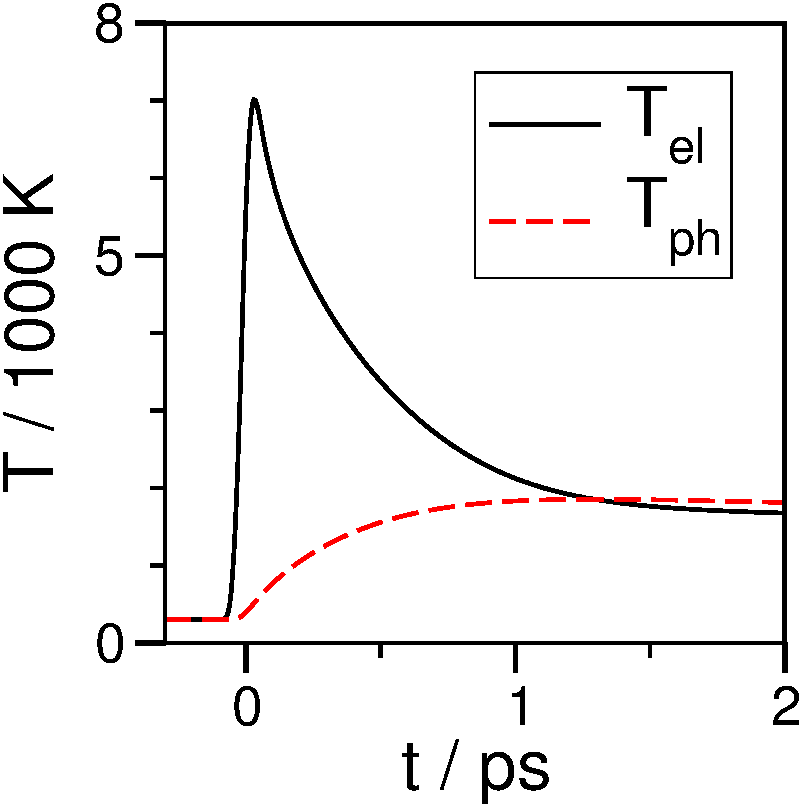
\includegraphics[width=1\textwidth]{figures/TTM_1pulse-eps-converted-to.pdf}
  \end{figure} 
  \column{0.8\textwidth}
  \vspace*{-1cm}
  \begin{figure}
        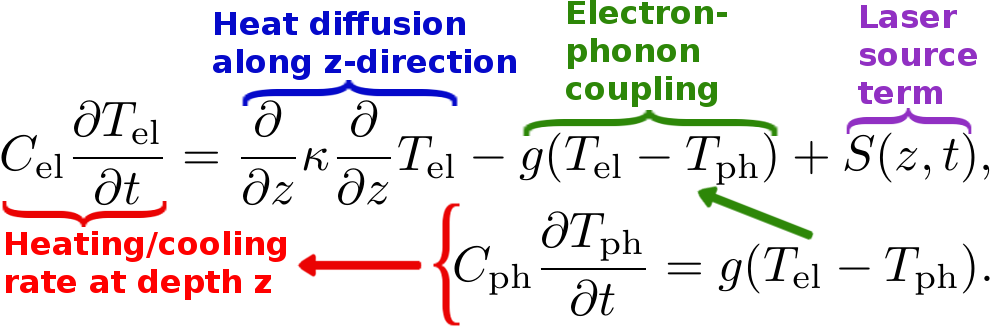
\includegraphics[width=\textwidth]{figures/2TM_equs.png}
  \end{figure}  
   \begin{block}{Original TTM {(\scriptsize Anisimov \textit{et al.}, \textit{SovPhys-JETP} 1974)} }
    \begin{itemize}
     \item $T_\mathrm{el}$ and $T_\mathrm{ph}$ as $f(z,t)$ {\footnotesize from laser/material properties}
     \begin{itemize}
     \footnotesize
     \item $C_\mathrm{el}$ and $C_\mathrm{ph}$ $\Rightarrow$ heat capacities
     \item $\kappa = \kappa_0 \frac{T_\mathrm{el}}{T_\mathrm{ph}}$ $\Rightarrow$ electron heat conductivity
     \item $g$ $\Rightarrow$ electron-phonon coupling constant
     \item $S(z,t)$ $\Rightarrow$ depends on pulse shape, $\lambda$, fluence $F$ 
          \end{itemize}
    \end{itemize}

   \end{block}
  \end{columns}
\end{frame}

\subsection[MDEF]{Electronic friction: non-adiabatic coupling approximated}
\begin{frame}{Different approaches to non-adiabatic coupling}
  \begin{figure}
        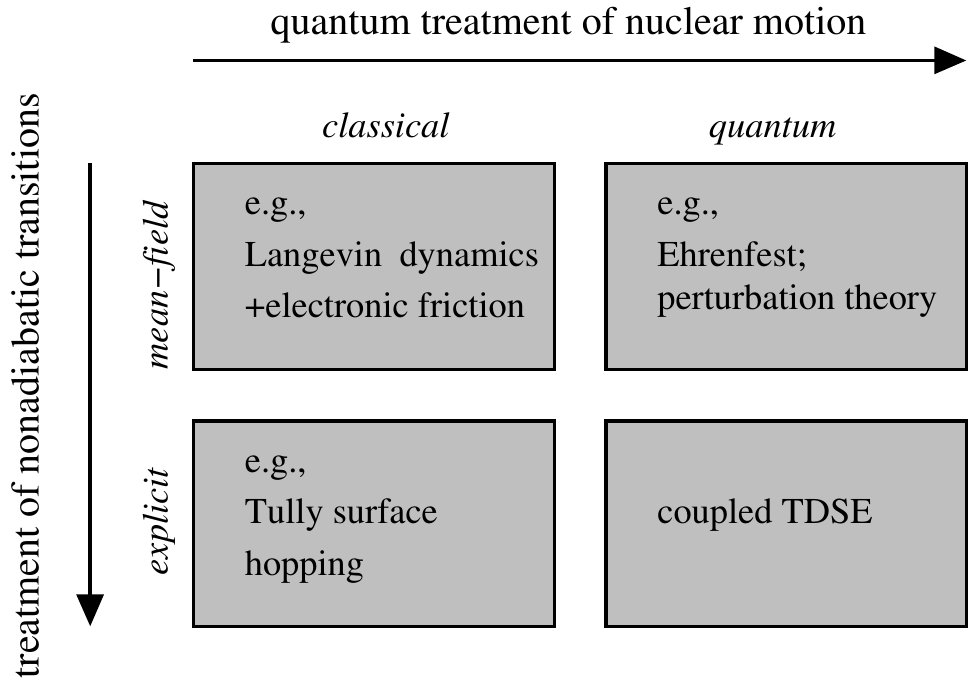
\includegraphics[width=.6\textwidth]{figures/scheme_nonadiab.png}
  \end{figure}
  \begin{block}{Langevin dynamics + electronic friction}
   \begin{itemize}
    \item fastest method $\Rightarrow$ suited for multi-dimensional dynamics
    \item good approximation for weak non-adiabatic coupling
   \end{itemize}

  \end{block}

\end{frame}

\begin{frame}{The Langevin equation}{A stochastic differential equation}
  \begin{columns}
  \column{0.3\textwidth}
   \begin{figure}
        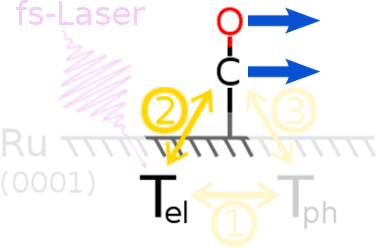
\includegraphics[width=\textwidth]{figures/Part2SurfScheme.png}
  \end{figure}
  \column{0.8\textwidth}
\begin{figure}
        
\includegraphics[width=\textwidth]{figures/Langevin_eq.png}
  \end{figure}
    \end{columns}
  \begin{block}{Langevin equation within IAA {\small(independent atom approx.)}}
  \begin{itemize}
   \item friction coefficient of Atom k: $\eta_{\mathrm{el},k}(\underline{r}_k)$ $\Rightarrow$ dissipation
  
      \begin{itemize}
      \footnotesize
      \item derived from local density friction approximation (LDFA)
      \newline $\Rightarrow$ individual atom (again IAA) in free electron gas
      \item $\eta_{\mathrm{el},k}(\underline{r}_k)$ dependent on electron density of bare surface
      \end{itemize}

    \item random force $\underline{R}_{\mathrm{el},k}(t)$ $\Rightarrow$ fluctuation% 
%     \item 
     
    \begin{itemize}\footnotesize
          \item Gaussian white noise
          \item describes excitation by hot electron-hole pairs
      \item proportional to: $\eta_{\mathrm{el},k}(\underline{r}_k)$ and $T_\mathrm{el}(t)$
    \end{itemize}
  \end{itemize}
  \end{block}
\end{frame}


\subsection[GLO]{The generalized Langevin oscillator (GLO)}
\begin{frame}[plain]{Generalized Langevin Oscillator}
  \begin{columns}[c]
    \column{0.25\textwidth}
          \vspace{-1.9cm}
          \begin{figure}
                \hspace*{-.7cm}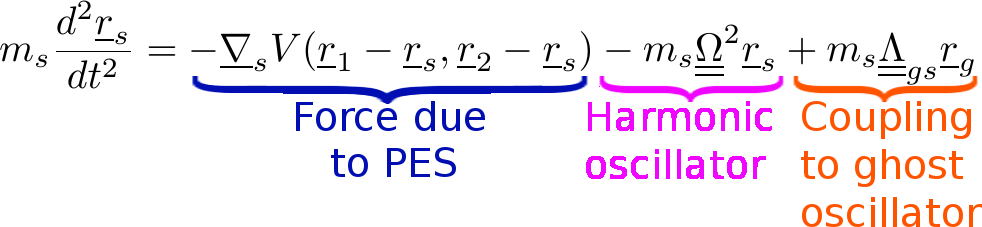
\includegraphics[width=2.6\textwidth]{figures/GLO_eq1.png}
          \end{figure}
          \begin{figure}
                \hspace*{-.7cm}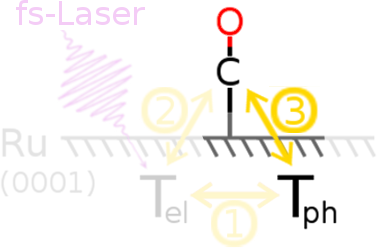
\includegraphics[width=1.3\textwidth]{figures/Part3SurfScheme.png}
          \end{figure}
          \vspace{-1cm}
          \begin{figure}
                \hspace*{-.7cm}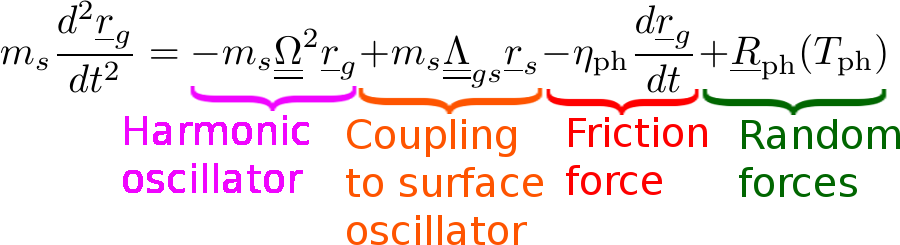
\includegraphics[width=2.4\textwidth]{figures/GLO_eq2.png}
          \end{figure}
        \column{.68\textwidth}
%         \begin{figure}
                \hspace*{-.7cm}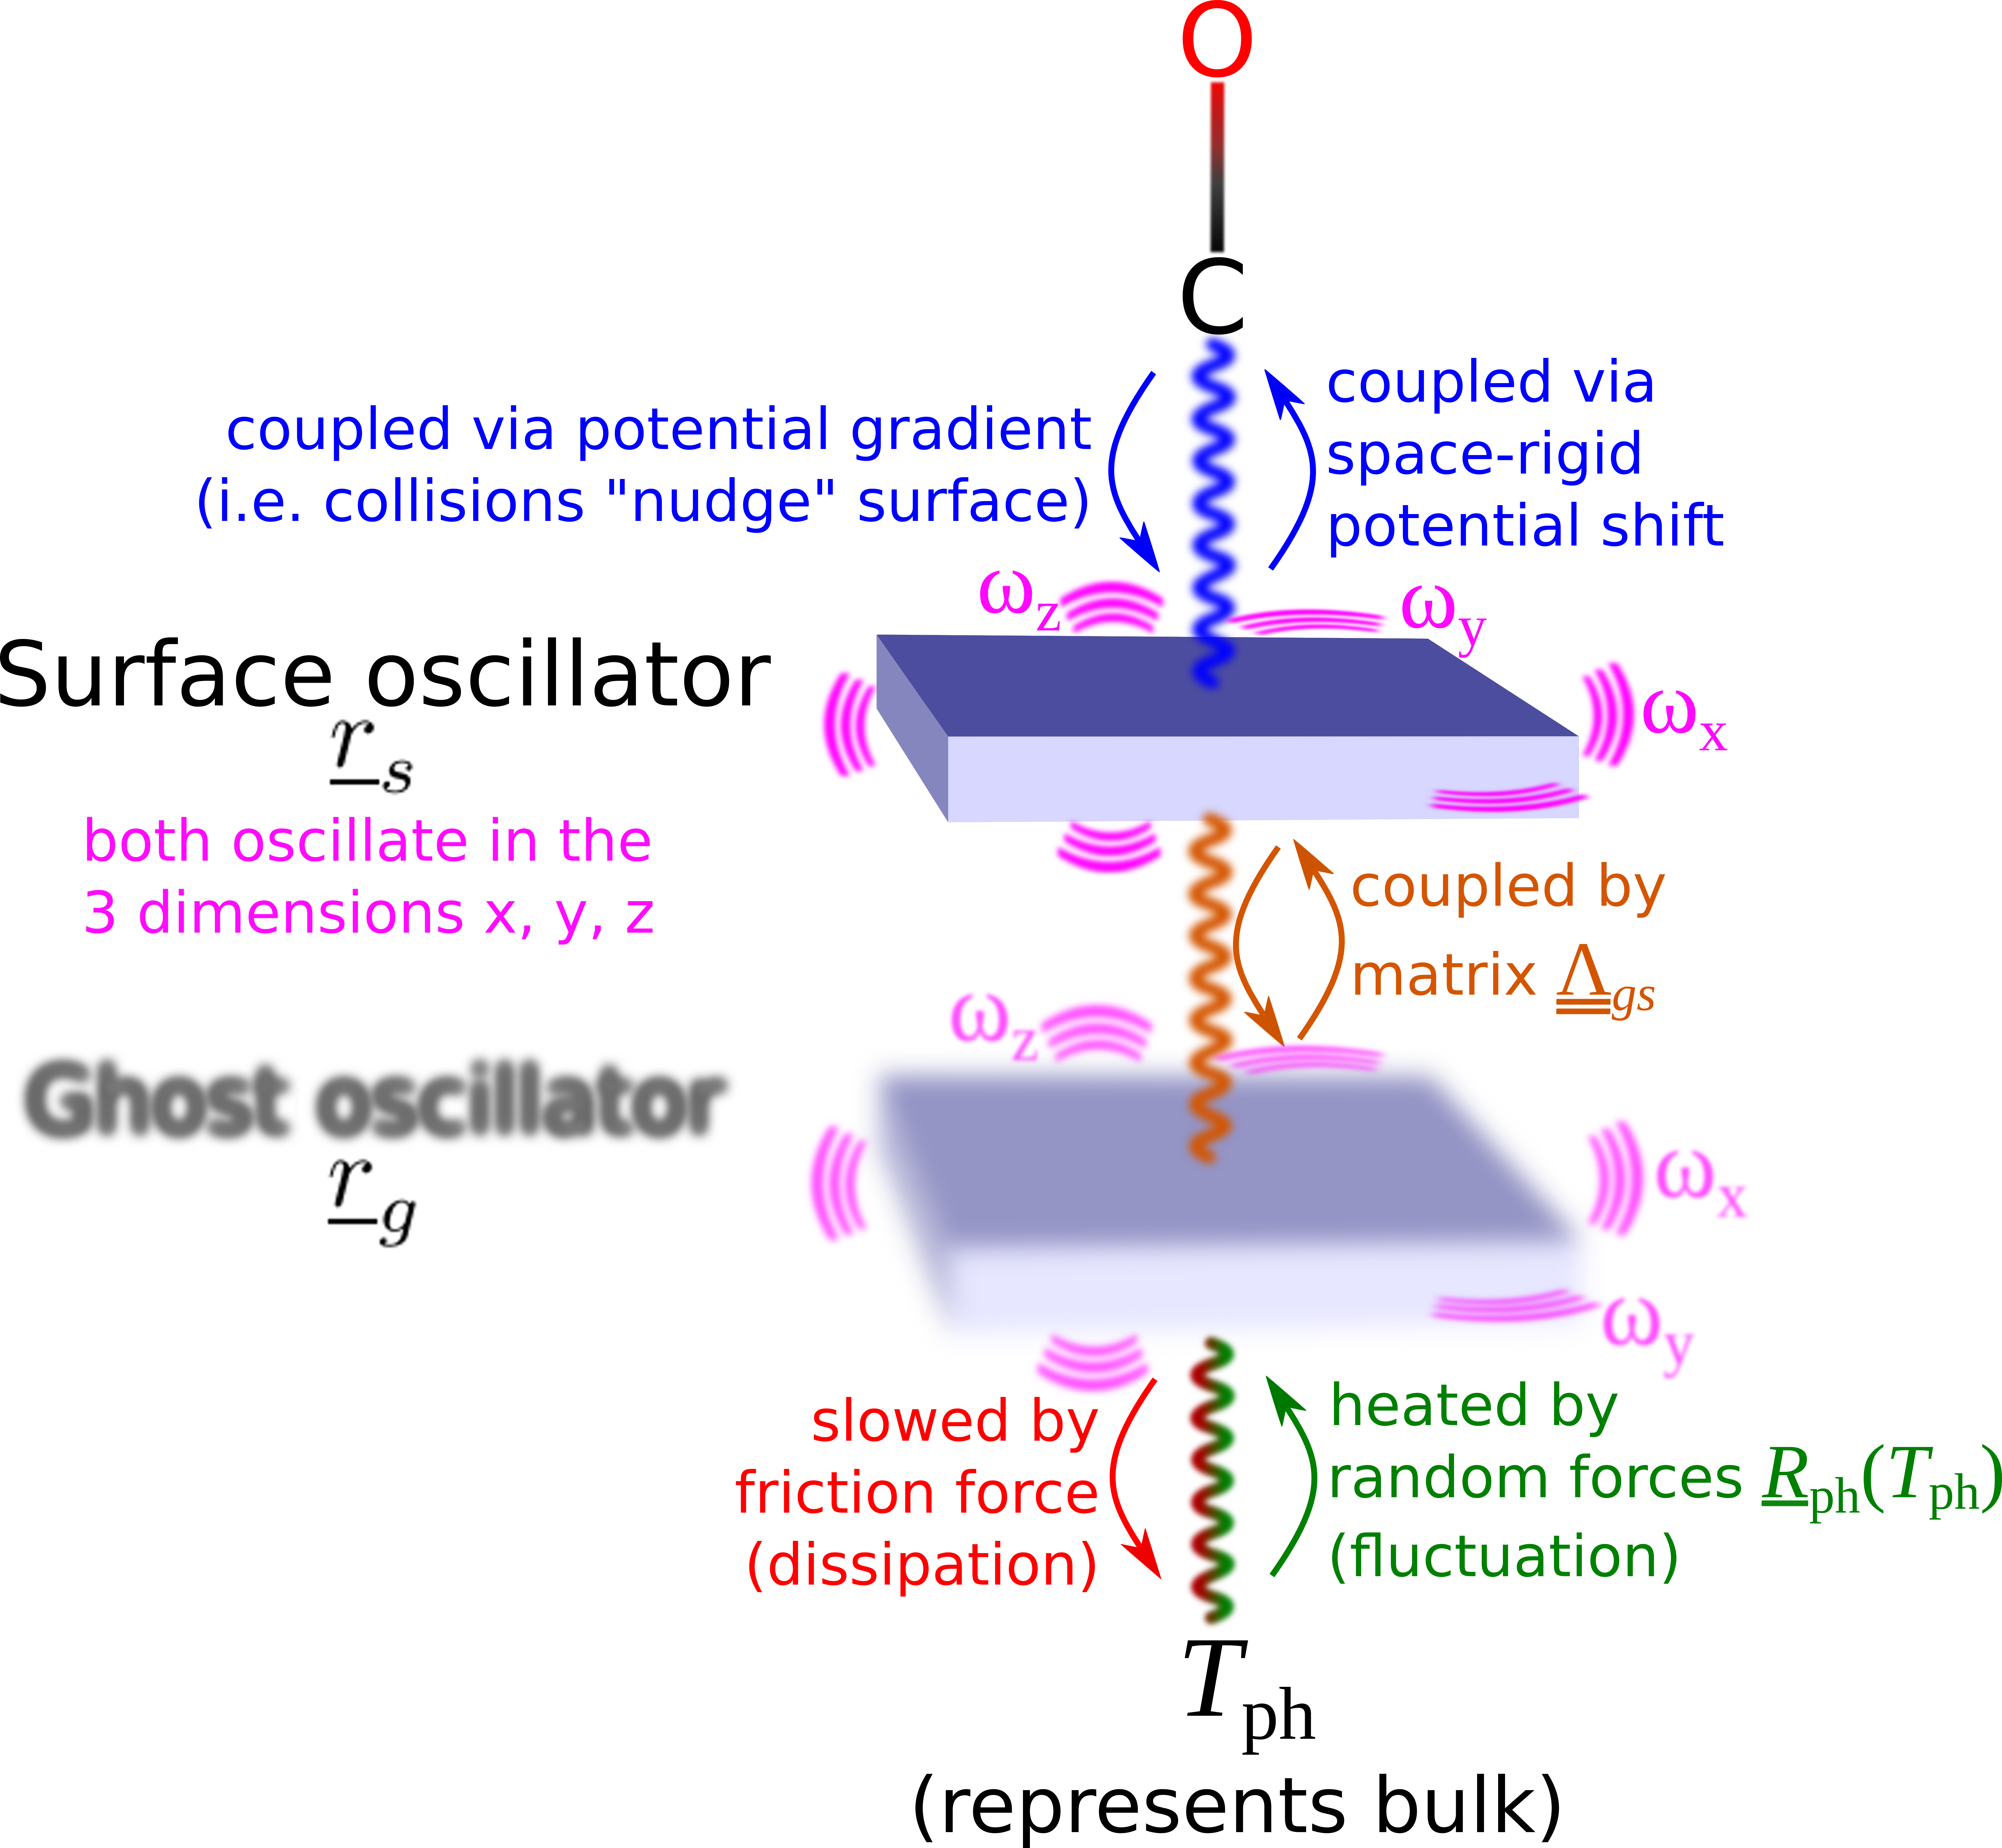
\includegraphics[width=1.2\textwidth]{figures/GLO.png}
%         \end{figure}
  \end{columns}
\end{frame}

\begin{frame}{Summary of models and methods}
  \begin{figure}
        \hspace*{-.85cm}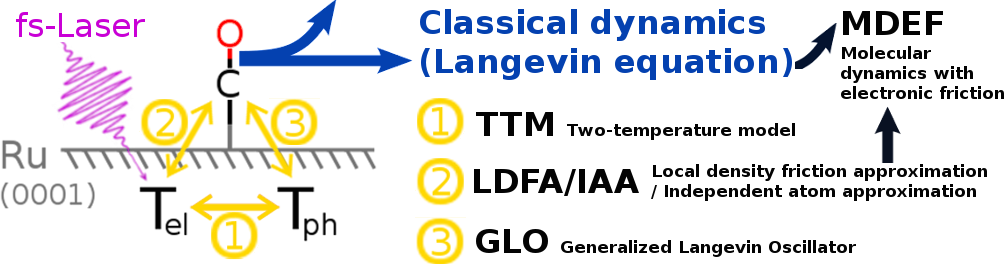
\includegraphics[width=1.15\textwidth]{figures/SummSurfScheme.png}
  \end{figure}
\end{frame}


\begin{frame}{Heating of DOFs $Z$ and $\theta$}
  \begin{figure}
        \vspace*{-.4cm}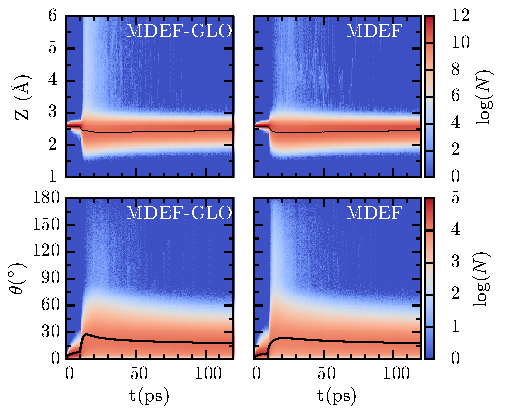
\includegraphics[width=.9\textwidth]{figures/ZundTheta.pdf}
  \end{figure}
\end{frame}

\begin{frame}{No population of physisorbed state in our dynamics}{As is to be expected from negligible barrier in potential of mean force (PMF)}
  \begin{columns}
  \column{0.6\textwidth}
    \begin{figure}
      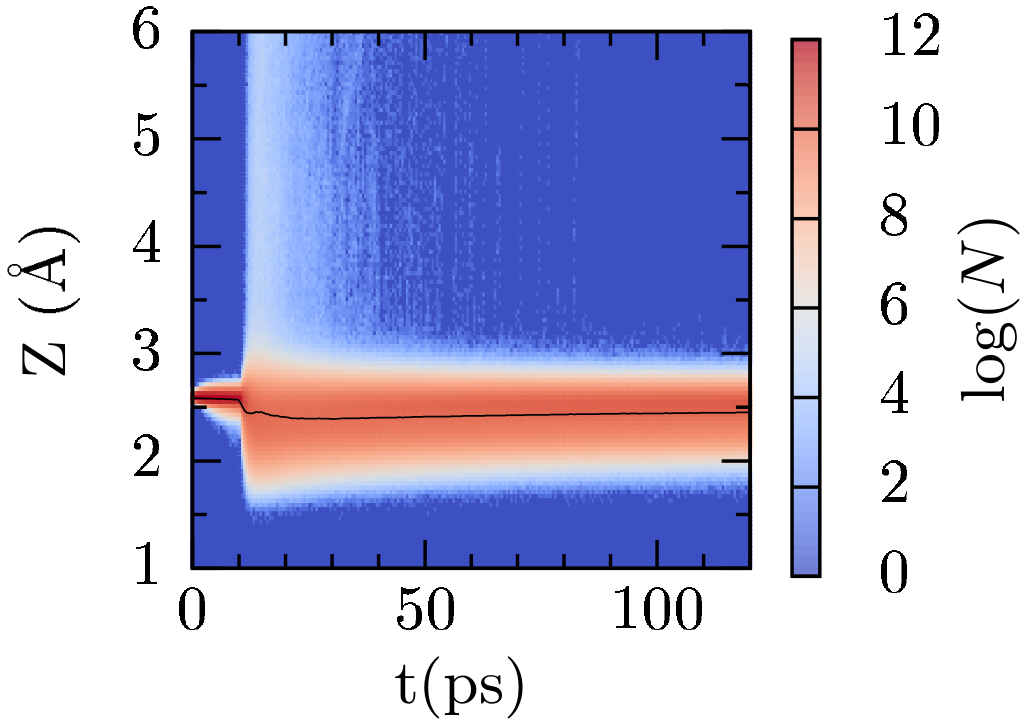
\includegraphics[width=1.\textwidth]{figures/NurZ.png}
    \end{figure}
  \column{0.4\textwidth}
    \begin{figure}
      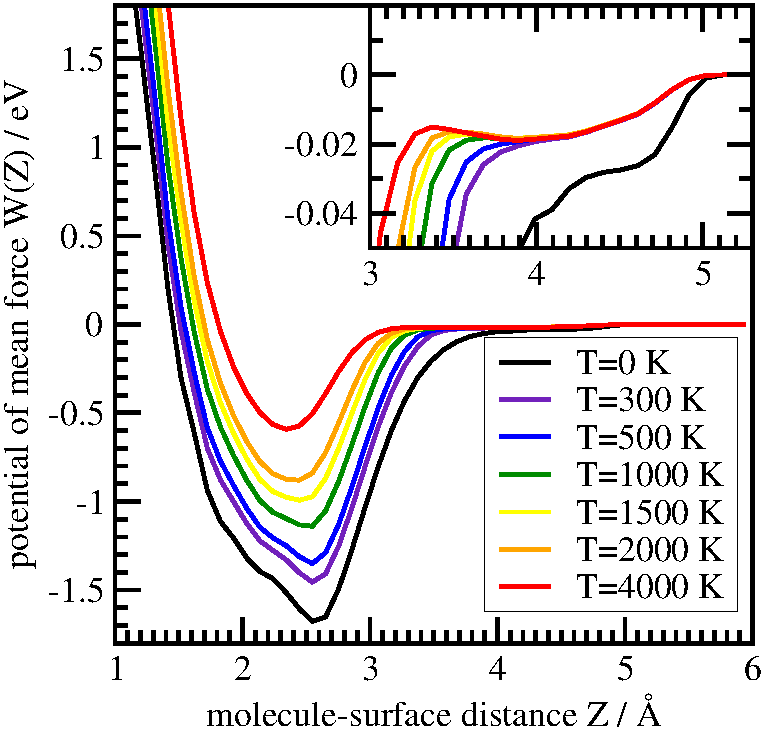
\includegraphics[width=1.\textwidth]{figures/GernotPMF.pdf}
    \end{figure}
  \end{columns}
\end{frame}

\begin{frame}{Why are the entropic barriers of the PMFs so different?}
  \begin{block}{Because separability assumption fails clearly}
    \begin{itemize}
     \item if introduced for our PMF $\Rightarrow$ barrier of similar heigth!
     \item expectable, because $X/Y$ and $\theta$ strongly coupled
    \end{itemize}
  \end{block}
  \begin{columns}
    \column{0.5\textwidth}
    \begin{figure}
      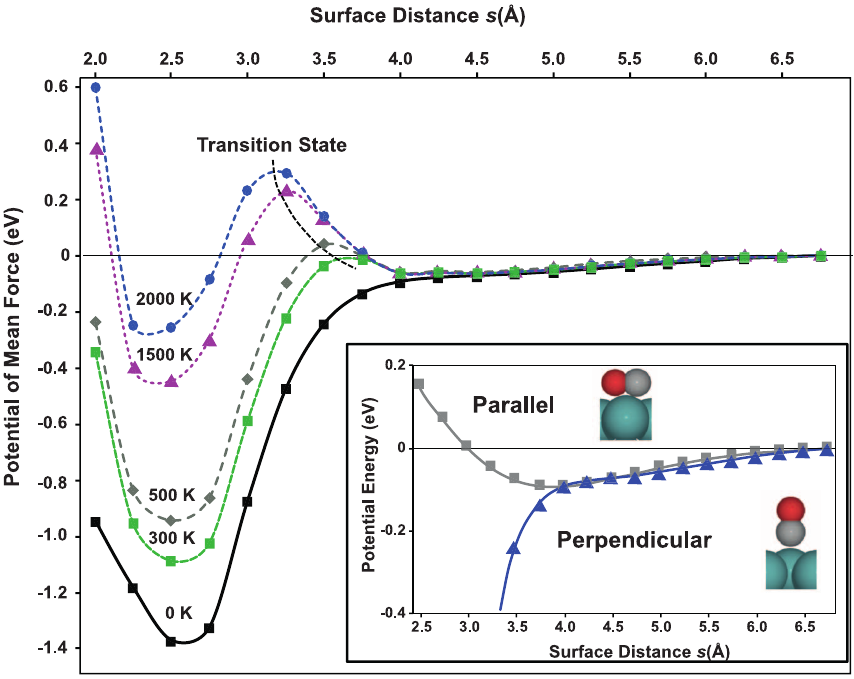
\includegraphics[width=\textwidth]{figures/sciencePMF.png}
    \end{figure}
    \column{0.5\textwidth}
    \begin{figure}
      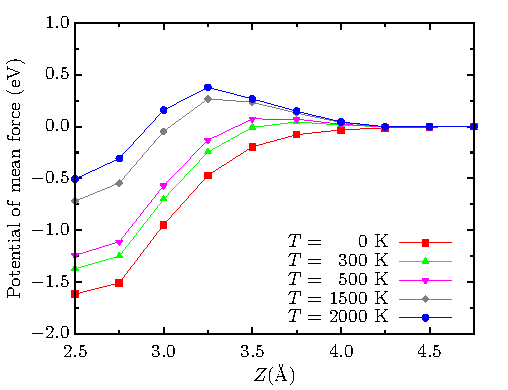
\includegraphics[width=\textwidth]{figures/PMF_Supp.pdf}
    \end{figure}   
  \end{columns}
\end{frame}



\begin{frame}{Dynamical trapping: {\normalsize alternative/additional explanation?}}

%     \begin{figure}
      \hspace*{-.6cm}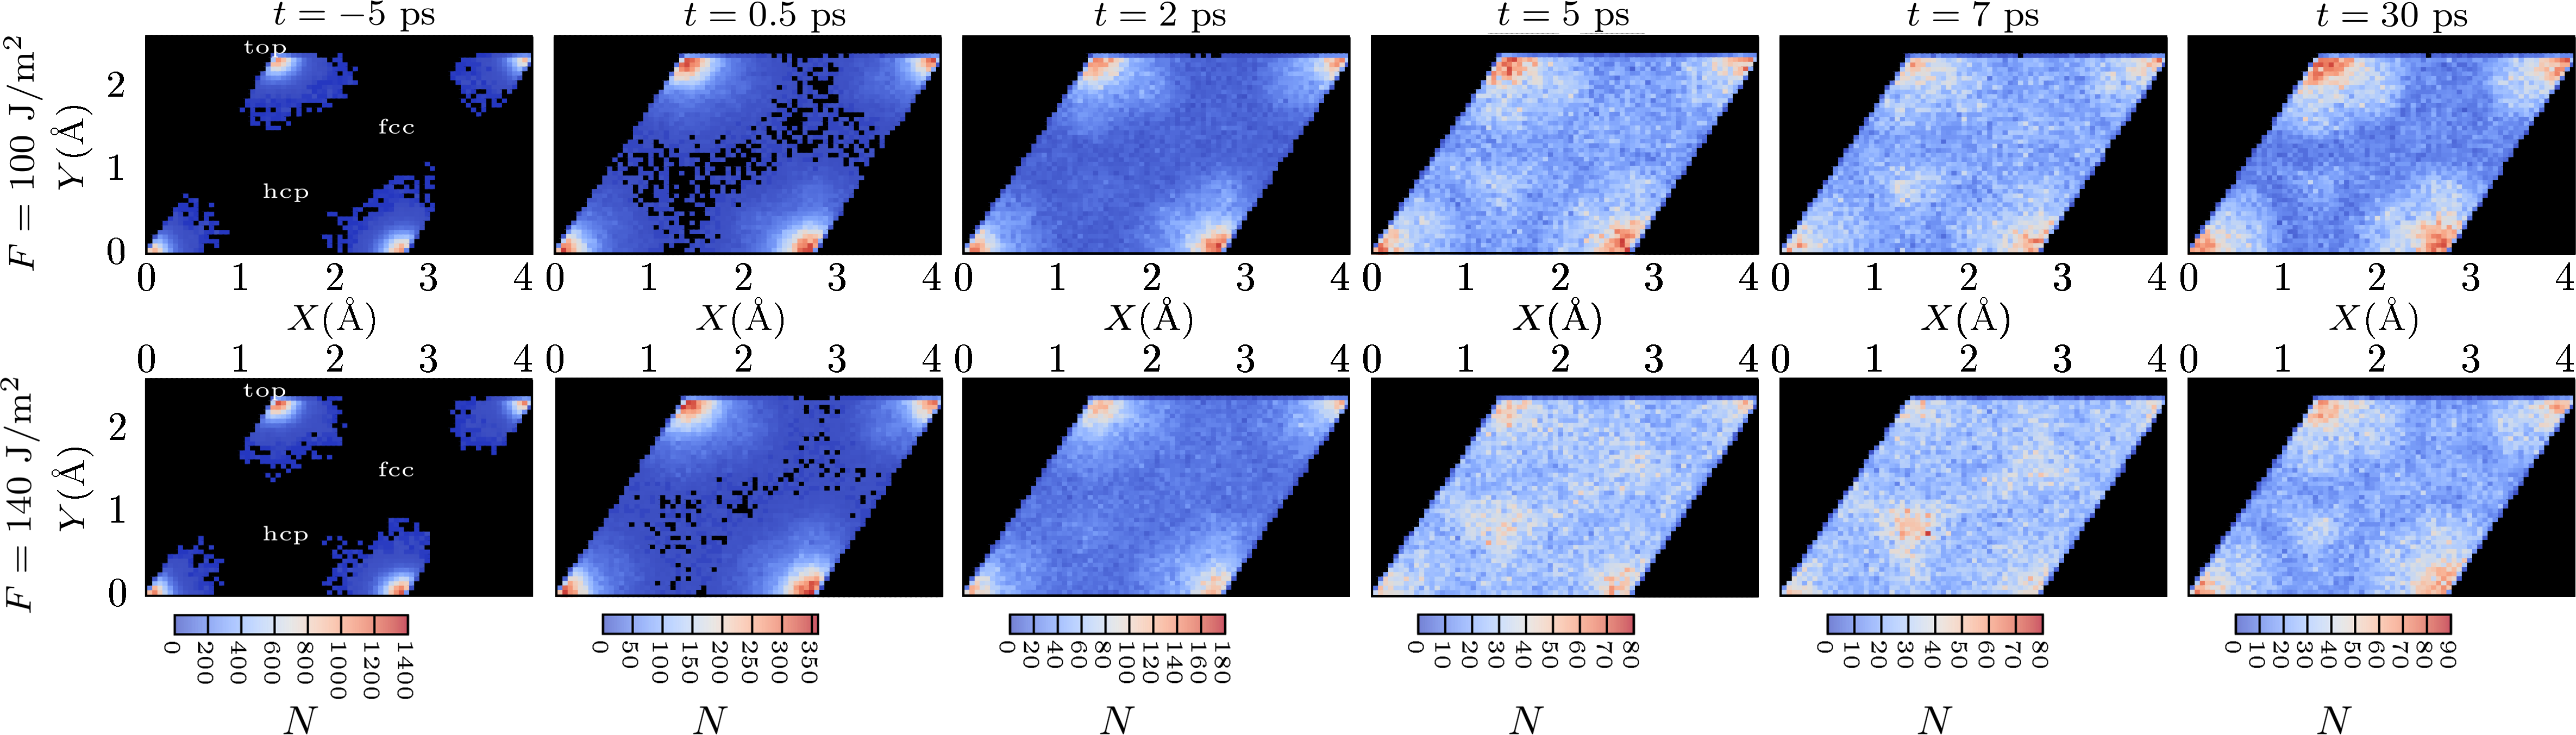
\includegraphics[width=1.1\textwidth]{figures/XYoverTime.png}
%     \end{figure}
\vspace*{-.5cm}
      \begin{columns}[t]
  \column{.65\textwidth}
  \begin{block}{Suprising patterns in XY-distribution}
    \begin{itemize}       
      \item preferation of \textbf{hcp-site} after 5-7$\,$ps,
%       \item[$\Rightarrow$] 
      \newline despite it being a local maximum!
      \newline \textbf{$\Rightarrow$ dynamical trapping} {\footnotesize(cf. 30$\,$ps)}
      \item effect dependent on fluence
      \newline $\Rightarrow$ consistent with experiment \newline{\footnotesize(weaker ``precursor''-signal for lower fluence)}
    \end{itemize}   
  \end{block}

  \column{.4\textwidth}
    \begin{figure}
      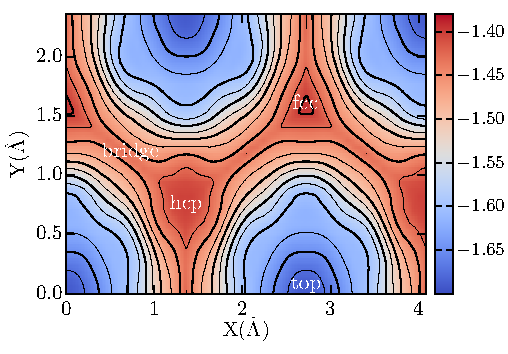
\includegraphics[width=\textwidth]{figures/PES_XYview.pdf}
    \end{figure}
  \end{columns}  
\end{frame}

\begin{frame}{Is there a physisorbed precursor state nevertheless?}
  \begin{columns}
    \column{0.7\textwidth}
    \begin{figure}
      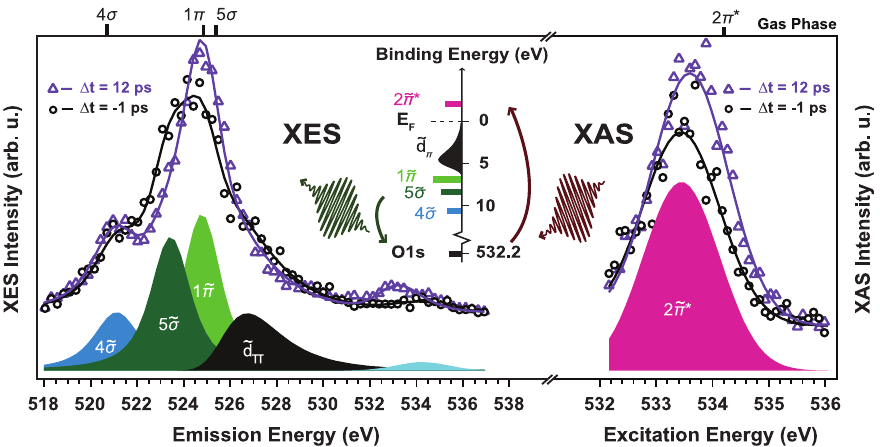
\includegraphics[width=1.\textwidth]{figures/scienceXray.png}
    \end{figure}      
    \column{0.2\textwidth}
    \begin{figure}
      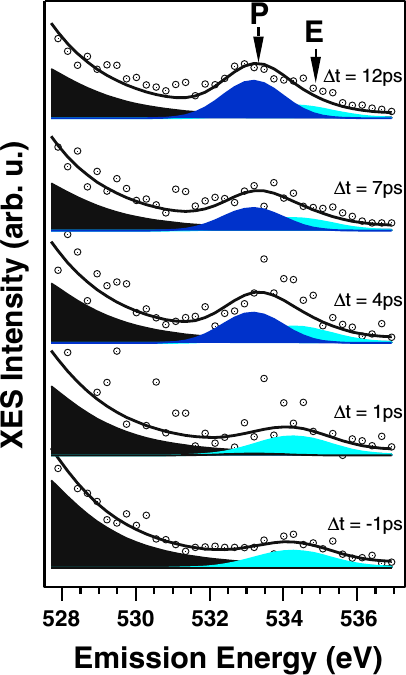
\includegraphics[width=1.\textwidth]{figures/PartiPeak.png}
    \end{figure} 
  \end{columns}
    \begin{block}{Dynamical trapping can't explain all observations}
      \begin{itemize}
        \item XAS of hcp-site: 2$\pi^*$-intensity not increased {\scriptsize(computed by Christopher)}
        \item participator peak not explained by any XY-redistributions
        \newline $\Rightarrow$ Existence of physisorbed state very likely
          \item but nevertheless not stable for Ru(2x2):CO models 
         \newline $\Rightarrow$ probably stabilized by CO-CO-interactions 


        
      \end{itemize}
    \end{block}
\end{frame}

\begin{frame}{Summary}
  \begin{block}{What was done?}
   \begin{itemize}
    \item 6D Langevin dynamics of CO @ Ru(0001)
    \begin{itemize}\scriptsize
    \item electronic friction and excitation by hot e-h-pairs (via LDFA/IAA)
    \item substrate motion (via GLO)
    \item based on ab-initio potential and first-principles, no ``free parameters''
    \end{itemize}  
   \end{itemize}

  \end{block}

  \begin{figure}
        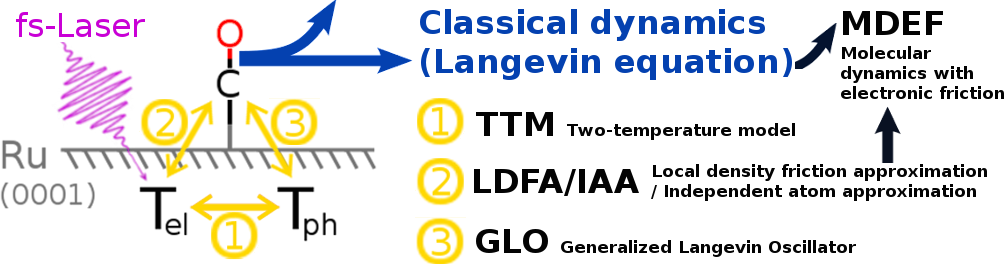
\includegraphics[width=0.85\textwidth]{figures/SummSurfScheme.png}
  \end{figure}
  \begin{block}{What could be learned?}
   \begin{itemize}
    \item detailed time- and space-resolved insight 
    \item physisorbed precursor state not stable in current model
   \end{itemize}

  \end{block}
\end{frame}

\begin{frame}{Outlook}{What can be done in the future?}
  \begin{block}{On the CO/Ru-system}
     \begin{itemize}
      \item better TTM, {\footnotesize with accurate $\kappa(T_\mathrm{el}, T_\mathrm{ph})$ and $g(T_\mathrm{el}, T_\mathrm{ph})$ (e-e-scattering) }  
      \item better friction model, {\footnotesize  e. g. LDFA with Atoms in Molecules (AIM)}
      \item use AIMDEF {\footnotesize to revisit short timescales of phonon-adsorbate coupling predicted by GLO}
      \item include CO-CO-interactions, \newline {\footnotesize e. g. via tailored FF for electrostatic and VdW-interactions \newline$\Rightarrow$ also enables simulation of other coverages} 
     \end{itemize}
   
  \end{block}
  \begin{block}{MDEF/GLO and AIMDEF on other systems}
    e.g. NO/Au(111), H$_2$/Au(111) etc.
  \end{block}

  
\end{frame}

  
% \begin{frame}[plain]{Outline}
%   \tableofcontents
%   % Die Option [pausesections] k�nnte n�tzlich sein.
% \end{frame}



% Da dies ein Vorlage f�r beliebige Vortr�ge ist, lassen sich kaum
% allgemeine Regeln zur Strukturierung angeben. Da die Vorlage f�r
% einen Vortrag zwischen 15 und 45 Minuten gedacht ist, f�hrt man aber
% mit folgenden Regeln oft gut.  

% - Es sollte genau zwei oder drei Abschnitte geben (neben der
%   Zusammenfassung). 
% - *H�chstens* drei Unterabschnitte pro Abschnitt.
% - Pro Rahmen sollte man zwischen 30s und 2min reden. Es sollte also
%   15 bis 30 Rahmen geben.
% 
% 
\end{document}

